\section{Подготовительная часть}
	В чем заключается суть данной работы? С концептуальной стороны вопроса ответ очевиден: дан временной ряд, необходимо предсказать его следующее значение наиболее точным образом. Но прежде чем перейти к рассмотрению использованных моделей,  формализуем поставленную задачу, ведь не всегда понятно, что имеется в виду под "наиболее точно"\ и "временной ряд".
	\subsection{Формализация проблемы}
		Пусть на вход программе, назовем ее $f$, подается временной ряд вида: $y_t: t = \overline{1,N}$. Пока что никаких предпосылок относительно данного временного ряда нет. Тогда задача алгоритма $f$ предсказать $\hat{y}_{t + 1}$ так, чтобы значение $|\hat{y}_{t + 1} - y_{t + 1}|$ было минимальным. То есть $f: \mathbb{R}^{N \times 1} \to \mathbb{R} \Rightarrow f(y) = \hat{y}_{t + 1}, \text{где } y = \left(y_1,\ldots,y_N\right)^T$. В терминах глубокого обучения, имеем задачу класса sequence to one \footnote{Sequence to one - задача получения одного значения, исходя из набора данных. К таким задачам относят: семантический анализ текста, классификацию картинок и так далее.} . \textbf{Q}: Но в принципе, что такое временной ряд? \textbf{A}: Временной ряд - это последовательность значений, относящихся к одному объекту в разные моменты времени. То есть, за тот период, когда за объектом наблюдали и снимали показатели. В нашем случае временной ряд - это набор доходностей акций за определенный период времени, то есть не ставится ограничение на знак данных величин, ведь она (доходность) может быть как отрицательной, так и положительной. \textbf{Q}: Почему именно доходности? \textbf{A}: Говоря о них, нет необходимости задумываться о том, сколько реально стоит та или иная акция/ценная бумага: $20$ руб. или $2\text{'}000$ руб. В анализе доходностей нас интересует: насколько они изменяются относительно некоторого момента времени. \textbf{Q}: Какого момента? \textbf{A}: Логично представлять доходность как прирост вида:
		\begin{equation}
			r_{t} = \frac{y_{t} - y_{t - 1}}{y_{t - 1}} = \frac{y_{t}}{y_{t - 1}} - 1
		\end{equation}
		То есть, как изменяется в процентах цена на некоторый актив (не обязательно акцию, хотя в нашем случае именно на нее) относительно предыдущего рабочего дня биржи. Однако внутри самой "акции"\ фигурирует несколько показателей, характеризующих ее в конкретный момент времени: цена открытия, максимальная и минимальная цены, цена закрытия, скорректированная цена закрытия и общая сумма сделок. Акцент делается на анализе цен открытия (так как с точки зрения автора работы важнее всего - хорошо начать рабочий день), хотя несомненно наличие взаимосвязи между ценой открытия и закрытия или иными доступными показателями. Когда есть возможность - другие показатели включаются в анализ, когда нет такой возможности (классическая модель не предназначена) - не включаются. Подводя итог: \textbf{Дано}: $y = \left(y_1, \ldots, y_n\right)^T$, \textbf{Найти}: $\hat{y}_{N + 1}: |\hat{y}_{N + 1} - y_{N + 1}| \to \min$. Подставляя вышеупомянутое равенство, имеем задачу оптимизации:
		\begin{equation}
			|f(y) - y_{N + 1}| \to \min_{\beta \in \mathbb{R}^k}
		\end{equation}
		Где $\beta$ - набор параметров модели, хотя некоторые из них имеют неоптимизируемые параметры (гиперпараметры), но в общем случае задача имеет подобный вид. Но проблема в том, что $y_{N + 1}$ неизвестно, а значит, невозможно подобрать алгоритм абсолютно точного прогнозирования, значит, необходимо на основе имеющейся информации сформировать алгоритм, который наиболее точным образом описывает предложенные ему данные, а далее делает предсказание, причем предсказание, как можно меньше отличающееся от реального значения. Только теперь, проведя подобные рассуждения, мы находимся в области машинного обучения и можем говорить о гипотезах рынка \footnote{Гипотезы рынка - обоснование исследования на качественном уровне, то есть утверждения о возможности проводить какой-либо технический анализ.} . Ведь для каждого типа рынка характерны свои особенности, следовательно, закономерный вопрос: почему мы вообще имеем право пытаться предсказывать что-то для развитой или развивающейся экономик. Изложение двух нижестоящих теорий представлено в сжатом виде, что делает повествование о них поверхностным, но достаточным для понимания всех особенностей работы.
		\subsubsection{Гипотеза эффективного рынка} \label{link::hypothsis_of_msrket_efficiency}
			Это одна из самых неоднозначных в плане количества последователей инвестиционная теория, ставящая своей целью описать принципы движения цен на активы, первоначальная версия которой "представлена"\ Луи Башелье в 1900 году. В его работе показана независимость доходности акций от течения времени, таким образом, Башелье пришел к выводу: "Вероятность роста цены в любой момент времени равна вероятности ее падения, а математическое ожидание спекулянта равно нулю". Много раз менявшая свою формулировку, начиная с Пола Самуэльсона: "На конкурентных рынках на всякого продавца найдется покупатель. Если можно быть уверенным, что цена вырастет, значит, она уже выросла"\ ,  в 1960-ых годах она (гипотеза) приобрела формальный вид в труде Юджина Фамы, использовавшего в исследованиях модель случайного блуждания, выведенную Башелье. По итогам эксперимента, Юджин Фама \cite{efficient_market} привел доказательство того, что вся доступная информация уже заложена в бумагах (позднее: "рынок полностью отражает всю доступную информацию"), то есть бесполезно пытаться предугадывать цены, любое предсказание не сбудется. Более того, единственный фактор, который способен повлиять на цену - это выходящие в будущем новости. А значит, перманентное доминирование над рынком не является возможным, а активное инвестирование не является состоятельным. Более подробная информация изложена в статье от 13 сентября 2022 года \cite{fama_market_efficiency}. На данный момент существует 3 основных гипотезы эффективности рынка:
			\begin{enumerate}
				\item \textbf{Слабая гипотеза} - в цене содержится вся историческая информация об активе и только фундаментальный анализ иногда может обеспечить избыточную доходность.
				\item \textbf{Полусильная гипотеза} - в ценах содержится вся публичная информация, таким образом, избыточную доходность может обеспечить только закрытая от широкой публики информация (инсайдерская).
				\item \textbf{Сильная гипотеза} - в ценах содержится как общедоступная, так и закрытая информация. Таким образом, ничто не может дать инвесторам избыточную доходность по сравнению со среднерыночным показателем.
			\end{enumerate}
			Тогда напрашивается вывод: если быть сторонником ГЭР, то настоящая работа не имеет смысла, ведь технический анализ не может дать дополнительной доходности для любой степени ее силы. Однако, по словам Мартина Свэлла, проанализировавшего историю данной гипотезы в работе \cite{matrin_swell}: "Строго говоря, гипотеза [прежде всего, в ее сильной форме] ложна, но по духу глубоко верна $\ldots$ До тех пор, пока текущая гипотеза не будет заменена лучшей гипотезой, критика имеет ограниченную ценность". Отсюда все-таки следует обоснование, почему существует так много математических моделей, пытающихся прогнозировать доходность активов. Отсюда следует, что в современном мире количество методов предсказания настолько велико, что исследователю сложно выбрать нужный, это еще одно подтверждение, почему настоящая работа имеет смысл.
		\subsubsection{Гипотеза фрактального рынка}
			Часто в качестве доказательства ложности ГЭР приводятся в пример финансовые кризисы, так как по ГЭР вероятность возникновения подобного кризиса пренебрежимо мала или приблизительно ноль. Таким образом, появляется еще одна гипотеза: Гипотеза Фрактального Рынка (ГФР), чьим родоначальником является Бенуа Мандельброт \cite{benoit_mandelbrot}, по которой можно объяснять кризисы. Ее основные характеристики: 1) график доходностей активов имеет фрактальную (всегда $1 < D <2$) размерность 2) Различные окна (интервалы) исходного графика могут быть самоподобными 3) Каждому финансовому графику присуща своя уникальная структура и соответственно ее свойства 4) Финансовый график обладает памятью о своих исходных условиях (имеет долгосрочную память; формальный способ проверки данного утверждения вводится позже). Для выполнения данной гипотезы предполагается, что рынок является стабильным, если он включает в себе очень много инвесторов с различными горизонтами планирования (это гарантия ликвидности). Объяснение кризисов происходит следующим образом, описанным в статье Палювиной А.С. \cite{fractal_market}: "Когда инвесторы меняют свои инвестиционные горизонты (например, фундаментальная информация становится ненадёжной, а	долгосрочные инвесторы уходят с рынка или сокращают свои горизонты),	баланс между краткосрочной и долгосрочной перспективами искажается,	рынок становится менее ликвидным и возникает кризис". Таким образом, из данной гипотезы следует вывод, что информационный и инвестиционный горизонты оказывают влияние на поведение инвестора.
		\subsubsection[Проверяемая гипотеза]{Проверяемая гипотеза настоящего исследования}
			Гипотеза, подтверждение которой настоящая работа ставит одной из своих ключевых задач, заключается в проверке суждения, что нейросетевой (далее NN) поход является наиболее эффективным применительно к исследуемой области финансовых рынков, а точнее к временным рядам цен/доходностей акций. То есть главный вопрос: нейросеть лучше справляется с прогнозированием доходностей акций по цене открытия на один рабочий день биржи по сравнению с другими использованными моделями или нет?
	\subsection{Наиболее популярные методы решения}
		В настоящем исследовании последовательно рассматриваются такие модели как: Exponentially Weighted Moving Average, Auto-regressive Integrated Moving Average, Generalized Auto-Regressive Conditional Heteroskedasticity, Auto-regressive Fractionally Integrated Moving Average, Fractionally Integrated GARCH, Singular Spectrum Analysis, Fourier \& Wavelet analysis, а также Transformers и моделирование сезонности. Далее рассказывается подробнейшим образом о математической подоплеке каждой из моделей. Важно понимать, что у данной работы нет задачи предоставить полноценное обоснование, почему та или иная модель однозначно работает, однако где-то все-таки приводится подробное описание, а где-то лишь качественные рассуждения и ссылки на более подробное обоснование. Сразу стоит отметить, обращаясь к последнему пункту плана (Transformers и моделирование сезонности), что он рассматривается с точки зрения: почему он тут не нужен \cite{transformers_are_useless_for_TSF}, несмотря на революцию в Natural Language Processing, устроенную методом self-attention \cite{attention_transformers} и несмотря на важный аспект моделирования временных рядов - сезонность. Механизм self-attention создан для вычленения смысла из данных. То есть: дан набор слов, к ему в соответствие ставится вектор (она называется embedding), а после к данному набору чисел применяются известные алгоритмы ML или DL. Однако в текущей задаче в ряде доходстей или цен (одно можно получить из другого) нет контекста, то есть и сам механизм теряет свою значимость. Трансформеры оперируют понятием контекста, отвечающего за связь слова с окружающими его словами. Математически-интуитивно это можно рассматривать следующим образом: $\{w_j\}_{j=1}^n$ - все предложение, смотрим на конкретное слово (не в начале и не в конце: между словом и концом/началом должно быть как минимум еще одно слово) $w_i: i \in (1,n)$. Контекстом данного слова называется набор $w_k: k \in \{i - l, \ldots, i - 1, i + 1, \ldots, i + l\}: l \in \N$. тут пропущено само слово, так как для него окно одного размера влево и вправо является контекстом. Это значит, что при таком последовательном выборе контекста необходимо максимизировать вероятность получения конкретного слова $w_i$. Данная задача ставится в процессе создания качественного эмебддинга (сопоставления чисел словам; алгоритм Word2Vec \cite{word2vec_2013}), но в текущей задаче нет необходимости рассматривать такую смысловую взаимосвязь между величинами ряда, так как, исходя из качественных рассуждений, на вход подается единственное число, которое никак, с точки зрения смысла, не связано с другими. Исходя из этого и делается вывод, что механизм трансформеров проигрывает более простым линейным моделям \cite{transformers_are_useless_for_TSF}. Что касается сезонности, то, несмотря на подтверждение ее наличия в финансовых временных рядах \cite{seasonality_in_financial_TS_is_real}, все-таки рассматриваем модели без корректировки на данную составляющую. Подобное рассуждения приводится, опираясь на Гипотезу Эффективного Рынка, утверждающую, что финансовые временные ряды не зависят от времени, иначе рынок перестал бы быть эффективным \cite{seasonality_test_for_financial_stock_market}. Данное суждение весьма прозаично относительно показанного факта в блоке \ref{link::hypothsis_of_msrket_efficiency} о некорректности всей гипотезы в целом. В итоге получается, что из ГЭР рассматривается (принимается как верное) только суждение об отсутствии сезонности, а все остальные положения принимаются как ложные. Таким образом, в данной работе не рассматриваются как Трансформеры, так и сезонность ряда (даже если эта составляющая присутствует, то она все равно относится к шуму). Далее приступаем к описанию моделей, рассматриваемых в настоящей работе. Для удобства делим их на требующие стационарность и не требующие. \textbf{Q}: Что такое стационарность? \textbf{A}: Существует определение как для случая, когда 1) временной ряд воспринимается как последовательная реализация случайных величин как-то распределенных, так и для случая, когда 2) временной ряд - некоторый сигнал, например, от светодиода или от звукового динамика. Последовательно:
		\begin{enumerate}
			\item Временной ряд - реализация набора зависимых случайных величин с различным - изменяющимся во времени - распределением. Случайная выборка - простейший частный случай для временного ряда, так как все полученные данные являются следствием реализации не одной случайной величины с некоторым распределением, а некоторого набора. Данные распределения заранее неизвестны и их пока что не представляется физической возможности определить, так как для их определения необходимо было бы посетить параллельную вселенную, где данная величина реализовалась бы иначе. То есть для максимальной точности потребовалось бы посещения $n \to \infty$ параллельных вселенных. Отсюда и возможность оперировать только частными случаями временных рядов - случайной выборкой. Таким образом, под всеми последующими упоминаниями термина "временной ряд"\ понимается термин "случайная выборка"\ - частный случай реализации временного ряда. Для данного определения существуют 2 понятия стационарности: в узком (сильном) и в широком (слабом) смыслах. Взяты из работы  Н. В. Артамонова, Е. А. Ивина \cite{stationarity_of_time_series_econometrics}, но переработаны для удобства восприятия.
			\begin{definition} \label{def::strong_ts_stationarity}
				\textbf{Если}: $\forall p, t_1, \ldots, t_p, l \in \mathbb{N} \Rightarrow$ распределение $y_{t_1}, y_{t_2}, \ldots y_{t_p}$ идентично распределению $y_{t_1 + l}, y_{t_2 + l}, \ldots, y_{t_p + l}$. \textbf{То}: Временной ряд называется стационарным в узком смысле (строго стационарным).
			\end{definition}
			\begin{definition} \label{def::weak_ts_stationarity}
				\textbf{Если}: $\forall t \in \mathbb{N} \Rightarrow \E(y_t) = \mu \in \R, \V(y_t) = \gamma_0, \cov(y_t, y_{t - k}) = \gamma_k: \mu, \gamma_0, \gamma_k$ не зависят от $t$. \textbf{То}: Временной ряд называется стационарным в широком смысле (слабо стационарным).
			\end{definition}
 			\item Временной ряд - просто набор чисел, содержащий информацию об объекте и полученный в ходе эксперимента (наблюдения за объектом). В этом случае стационарности дается следующее определение:
 			\begin{definition} \label{def::signal_stationarity}
 				\textbf{Если}: спектр амплитуд сигнала является постоянным во времени. \textbf{То}: Сигнал называется стационарным.
 			\end{definition}
 			В данном случае имеет место деление: стационарный, значит, либо детерминированный (то есть: однозначно определяется по некоторому закону и является периодическим/квазипериодическим/непериодическим), либо случайный (например, модели финансового рынка, основанного на Броуновском Движении \cite{brownian_motion_for_stochastic_differential_equation} или Белом шуме \cite{white_noise_for_stochastic_differential_equation}); нестационарный, значит, непрерывный или переходный. Более подробно о данном понятии и формальном его осознании рассказывается в блоках \ref{link::fourier_analysis} (Анализ Фурье) и \ref{link::wavelet_analysis} (Wavelet анализ).
		\end{enumerate}
		Исходя из вышеперечисленных определений, выделяем 2 группы моделей: стационарные и нестационарные. Стационарные модели - те, для которых необходимо выполнение предпосылки о слабой (стр. \pageref{def::weak_ts_stationarity} опр. \ref{def::weak_ts_stationarity}) или сильной (стр. \pageref{def::strong_ts_stationarity} опр. \ref{def::strong_ts_stationarity}) стационарности. Нестационарные - те, для которых нет строгой необходимости в этом (они могут работать как со стационарными данными, так и с нестационарными).		
		
		\subsubsection{Exponentially Weighted Moving Average} \label{link::ewma}
Предполагаем, что в наличии есть данные о некотором показателе $\theta_t: t = \overline{1,n}$. В данный момент перед нами не стоит задача предсказания следующего показателя, нужно только визуально выявить тренд, чтобы приблизительно понять направление движение показателя в осях (время, значение). Конечно, в этой формулировке отсутствует строгость, пока что останавливаемся на том, что есть. Экспоненциальная скользящая средняя занимается тем, что уже заложено в ее названии: сглаживает показатели посредством усреднения. То есть в текущем значении ($t$) используется как значение в предыдущий момент времени ($t - 1$), так и значение наблюдения в момент времени ($t$). Иными словами, получается выпуклая линейная комбинация текущего и предыдущего значений:
\begin{equation}
	v_t = \beta \cdot v_{t - 1} + (1 - \beta) \cdot \theta_t: \; \beta \in (0,1)
\end{equation}
Где $\beta$ - показатель, пропорциональный примерному количеству дней, по которым происходит усреднение, а $v_0 = 0$ - первое значение экспоненциальной скользящей средней. Для изучения данного рекуррентного соотношения "раскручиваем"\ его в обратном направлении:
\begin{equation}
	\begin{split}
		v_t & =  (1 - \beta) \cdot \theta_t + \beta \cdot \overbrace{\left\{(1 - \beta) \theta_{t - 1} + \beta v_{t - 2}\right\}}^{v_{t - 1}}\\
		& =  (1 - \beta) \cdot \theta_t + \beta \cdot \{(1 - \beta) \cdot \theta_{t - 1} + \beta \cdot \overbrace{\left\{(1 - \beta) \cdot \theta_{t - 2} + \beta \cdot v_{t - 3}\right\}}^{v_{t - 2}}\}\\
	\end{split}
\end{equation}
Для лучшего понимания, рассматриваем частный случае:
\begin{equation}
	\begin{split}
		v_4 & = \beta \cdot v_3 + (1 - \beta) \cdot \theta_4\\
		v_3 & = \beta \cdot v_2 + (1 - \beta) \cdot \theta_3\\
		v_2 & = \beta \cdot v_1 + (1 - \beta) \cdot \theta_2\\
		v_1 & = \beta \cdot v_0 + (1 - \beta) \cdot \theta_1\\
		v_0 & = 0
	\end{split}
\end{equation}
Тогда:
\begin{equation}
	\begin{split}
		v_4 & =  (1 - \beta) \theta_4 + \beta ((1 - \beta) \theta_3 + \beta ((1 - \beta) \theta_2 + \beta((1 - \beta) \theta_1 + \overbrace{\beta \cdot 0}^{v_0 = 0})))\\
		& = (1 - \beta) \theta_4 + (1 - \beta) \beta \cdot \theta_3 + (1 - \beta) \beta^2 \cdot \theta_2 + (1 - \beta) \beta^3 \cdot \theta_1\\
		& = (1 - \beta) \sum_{t = 1}^4 \beta^{4 - t} \cdot \theta_t
	\end{split}
\end{equation}
Аналогично происходит раскрытие и для больших показателей $v_n$. А значит, получается формула вида:
\begin{equation}
	v_n = (1 - \beta) \sum_{t = 0}^n \beta^t \cdot \theta_{n - t}
\end{equation}
Отсюда качественно делаем вывод, что последним значениям наблюдаемого показателя ($\theta$) соответствует большее значение коэффициента, то есть чем ближе $\theta_{t}$ к $v_n$ с точки зрения индекса, тем больше при нем коэффициент. Теперь, возвращаясь к названию модели, отмечаем, что она должна усреднять по конкретному количеству временных единиц, следовательно, $\beta$ (единственный гиперпараметр) должен регулировать указанный показатель (то есть количество дней, по которым происходит усреднение). Обычно, рассматривается следующее соотношение: $\beta = 1 - \alpha / (N + 1)$, где $N$ - количество дней, а $\alpha$ - фактор сглаживания. Опираясь на \cite{ewma}, полагаем $\alpha = 2$ как наиболее распространенное значение.

Далее рассматриваем подробнее первые значения EWMA, а конкретнее - для лучшего осознания - самое первое: $v_0 \Rightarrow v_1 = (1 - \beta) \cdot \theta_1 \Rightarrow$ при $\beta \to 1 - 0$ получаем, что $(1 - \beta) \cdot \theta_1 \ll \theta_1$, что крайне плохо отражается на самих значениях. Таким образом, вычленение тренда становится более трудным на начальных этапах из-за плохого "разогрева"\ модели. Данная проблема называет bias (смещение), а ее решение bias correction (коррекция смещения) соответственно. Основой подобной корректировки является множитель вида $(1 - \beta^t)$. Очевидно, что при $\beta \in (0,1)$, а именно так и есть по построению, $\lim\limits_{t \to +0}(1 - \beta^t) = 0$, а $\lim\limits_{t \to +\infty}(1 - \beta^t) = 1$.
\begin{equation}
	\begin{split}
		v_n & = (1 - \beta^n)^{-1} \cdot (\beta \cdot v_{n - 1} + (1 - \beta) \cdot \theta_n)\\
		v_n & = (1 - \beta^n)^{-1} \cdot (1 - \beta) \left(\sum_{t = 0}^n \beta^t \cdot \theta_{n - t}\right)
	\end{split}
\end{equation}
Тогда на начальных этапах коррекция выравнивает ранее сильно уменьшенные значения EWMA, а на последующих (при $n \to \infty$) ее влияние ослабеваем, постепенно сводясь к 0 (то есть - делению на 1). Данный способ занимает очень мало памяти компьютера, так как для вычисления ему всегда необходимо хранить только 2 переменные: $v_t$ и $\beta$.

Иллюстрируем вышеизложенную теорию на примере реальных данных. Рассматривается цена открытия акций компании Apple за 2021 год. Первоначально сами значения, представленные в координатах ($t$ - месяц года, $y_t$ - цена в рублях), имеют вид:
\begin{figure}[H]
	\centering
	\begin{tikzpicture}
		\begin{axis}[
			grid = both,
			legend pos = north west,
			minor tick num = 1,
			major grid style = {lightgray},
			minor grid style = {lightgray!25},
			xlabel = {2021 год},
			width = \textwidth,
			height = 0.5 \textwidth,
			xmin=-5, xmax=260,
			ymin=115, ymax=185,
			xtick={0, 40, 80, 120, 160, 200, 240},
			xticklabels={03/01, 02/03, 28/04, 24/06, 20/08, 18/10, 14/12},
			line width=0.3mm
			]
			\addplot table [
			x=x, 
			y=Open, 
			col sep=comma,
			mark={},
			] {./source/source_csv/Illustration data/apple_data_test.csv};
			\legend{AAPL 2021}
		\end{axis}
	\end{tikzpicture}
	\caption{Цены открытия акций Apple (AAPL) 2021 (руб.)}
\end{figure}
Исходя из графика, получаем, что данные очень нестабильны, то есть с первого взгляда невозможно точно сказать, каков тренд. Однако в общих чертах графика однозначно видно, что от малых значений цен показатели переходят к б\'{о}льшим. Применяем к данным модель EWMA.
\begin{figure}[H]
	\centering
	\begin{tikzpicture}
		\begin{axis}[
			grid = both,
			legend pos = north west,
			minor tick num = 1,
			major grid style = {lightgray},
			minor grid style = {lightgray!25},
			xlabel = {2021 год},
			width = \textwidth,
			height = 0.5 \textwidth,
			xmin=-5, xmax=260,
			ymin=115, ymax=185,
			xtick={0, 40, 80, 120, 160, 200, 240},
			xticklabels={03/01, 02/03, 28/04, 24/06, 20/08, 18/10, 14/12},
			line width=0.3mm
			]
			\addplot table [
			x=x, 
			y=Open, 
			col sep=comma,
			mark={},
			] {./source/source_csv/Illustration data/apple_data_test_ewma.csv};
			%\legend{AAPL 2021};
			
			\addplot table [
			x=x, 
			y=V_2, 
			col sep=comma,
			mark={},
			] {./source/source_csv/Illustration data/apple_data_test_ewma.csv};
			%\legend{EWMA $\beta = 0.1$};
			
			
			\addplot table [
			x=x, 
			y=V_10, 
			col sep=comma,
			mark={},
			] {./source/source_csv/Illustration data/apple_data_test_ewma.csv};
			%\legend{EWMA $\beta = 0.1$};
			
			\addplot table [
			x=x, 
			y=V_30, 
			col sep=comma,
			mark={},
			] {./source/source_csv/Illustration data/apple_data_test_ewma.csv};
			%\legend{EWMA $\beta = 0.3$};
			
			\addplot table [
			x=x, 
			y=V_50, 
			col sep=comma,
			mark={},
			] {./source/source_csv/Illustration data/apple_data_test_ewma.csv};
			%\legend{EWMA $\beta = 0.5$};
			
			
			\addplot table [
			x=x, 
			y=V_90, 
			col sep=comma,
			mark={},
			] {./source/source_csv/Illustration data/apple_data_test_ewma.csv};
			%\legend{EWMA $\beta = 0.9$};
			
			\addplot table [
			x=x, 
			y=V_200, 
			col sep=comma,
			mark={},
			] {./source/source_csv/Illustration data/apple_data_test_ewma.csv};
			%\legend{EWMA $\beta = 0.9$};
			
			\legend{AAPL 2021, $n = 2$, $n = 10$, $n = 30$, $n = 50$, $n = 90$, $n = 200$};
		\end{axis}
	\end{tikzpicture}
	\caption{EWMA, цены открытия AAPL 2021 (руб.)}
\end{figure}
Глядя на полученный результат сразу ясно, что тренд восходящий, однако это предположение делается только на основе визуального анализа. Пока что никаких алгоритмов нет. Однако нельзя недооценивать полученную информацию, так как более явный тренд позволяет моделям (нейронных сетей) более точно настраиваться на обучающую выборку, что часто приводит к улучшению результату предсказаний (если, конечно не довести до переобучения: данные термины и теория объясняется в блоке \myref{link::neural_networks}). Также стоит отметить всплеск, случившийся при $n = 2$. Это произошло именно именно из-за технических особенностей добавленного множителя, корректирующего смещение. 

Последним пунктом необходимо рассказать более подробно о самом корректирующем множителе. \textbf{Q}: Почему у него именно такой вид, ведь можно просто сделать первое значение таким же, как в исходном ряде? \textbf{A}: 1) необходимо корректировать вычисления, исходя из одной формулы, так как цель - прийти именно к общности 2) при последующих наблюдения данный коэффициент становится чрезвычайно малым $\lim\limits_{t \to +\infty}(1 - \beta^t) = 1$, а при первоначальных значениях не оказывает влияния $\lim\limits_{t \to +0}(1 - \beta^t) = 0$. Однако при индексах (речь о непрерывных), стремящихся к $0$, обратная величина стремится к $\infty$, что очень плохо с вычислительной точки зрения, так как у компьютера может произойти переполнение памяти и вместо числа получится NaN или Null, что не позволит далее осуществлять расчеты. Поэтому в начале графике наблюдается резкий всплеск, сходящийся впоследствии к исходному ряду. Далее приводится график значений корректирующих коэффициентов в зависимости от $\beta$ и от $t$.
\begin{figure}[H]
	\centering
	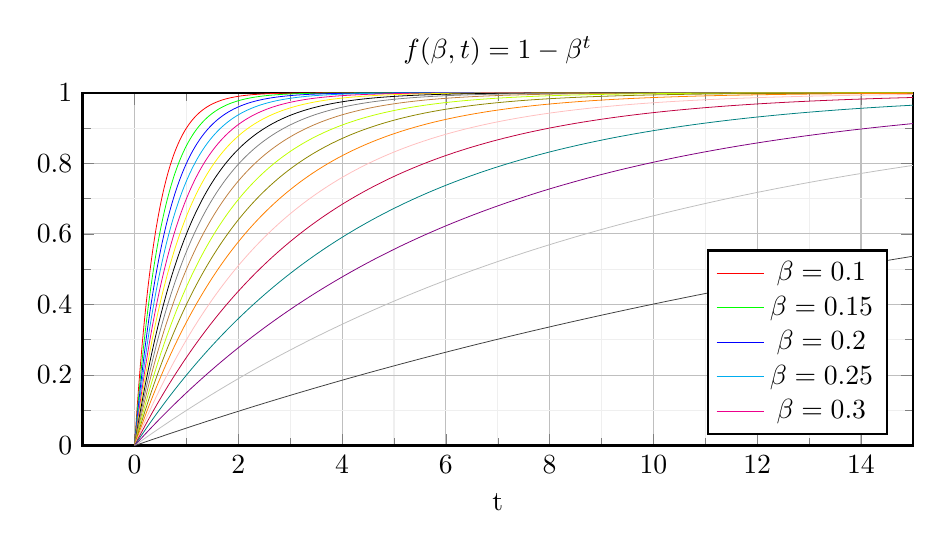
\begin{tikzpicture}
		\begin{axis}[
			grid = both,
			legend pos = south east,
			minor tick num = 1,
			major grid style = {lightgray},
			minor grid style = {lightgray!25},
			title={$f(\beta, t) = 1 - \beta^t$},
			xlabel = {t},
			width = \textwidth,
			height = 0.5 \textwidth,
			xmin=-1, xmax=15,
			ymin=0, ymax=1,
			%xtick={0, 40, 80, 120, 160, 200, 240},
			%xticklabels={03/01, 02/03, 28/04, 24/06, 20/08, 18/10, 14/12},
			line width=0.3mm
			]
			\addplot[domain = 0:15,
			samples = 300,
			color = red,
			smooth,
			line width = 0.01cm,] {1 - 0.1^x};
			\addplot[domain = 0:15,
			samples = 300,
			color = green,
			smooth,
			line width = 0.01cm,] {1 - 0.15^x};
			\addplot[domain = 0:15,
			samples = 300,
			color = blue,
			smooth,
			line width = 0.01cm,] {1 - 0.2^x};
			\addplot[domain = 0:15,
			samples = 300,
			color = cyan,
			smooth,
			line width = 0.01cm,] {1 - 0.25^x};
			\addplot[domain = 0:15,
			samples = 300,
			color = magenta,
			smooth,
			line width = 0.01cm,] {1 - 0.3^x};
			\addplot[domain = 0:15,
			samples = 300,
			color = yellow,
			smooth,
			line width = 0.01cm,] {1 - 0.35^x};
			\addplot[domain = 0:15,
			samples = 300,
			color = black,
			smooth,
			line width = 0.01cm,] {1 - 0.4^x};
			\addplot[domain = 0:15,
			samples = 300,
			color = gray,
			smooth,
			line width = 0.01cm,] {1 - 0.45^x};
			\addplot[domain = 0:15,
			samples = 300,
			color = brown,
			smooth,
			line width = 0.01cm,] {1 - 0.5^x};
			\addplot[domain = 0:15,
			samples = 300,
			color = lime,
			smooth,
			line width = 0.01cm,] {1 - 0.55^x};
			\addplot[domain = 0:15,
			samples = 300,
			color = olive,
			smooth,
			line width = 0.01cm,] {1 - 0.6^x};
			\addplot[domain = 0:15,
			samples = 300,
			color = orange,
			smooth,
			line width = 0.01cm,] {1 - 0.65^x};
			\addplot[domain = 0:15,
			samples = 300,
			color = pink,
			smooth,
			line width = 0.01cm,] {1 - 0.7^x};
			\addplot[domain = 0:15,
			samples = 300,
			color = purple,
			smooth,
			line width = 0.01cm,] {1 - 0.75^x};
			\addplot[domain = 0:15,
			samples = 300,
			color = teal,
			smooth,
			line width = 0.01cm,] {1 - 0.8^x};
			\addplot[domain = 0:15,
			samples = 300,
			color = violet,
			smooth,
			line width = 0.01cm,] {1 - 0.85^x};
			\addplot[domain = 0:15,
			samples = 300,
			color = lightgray,
			smooth,
			line width = 0.01cm,] {1 - 0.9^x};
			\addplot[domain = 0:15,
			samples = 300,
			color = darkgray,
			smooth,
			line width = 0.01cm,] {1 - 0.95^x};
			\legend{$\beta = 0.1$, $\beta = 0.15$, $\beta = 0.2$, $\beta = 0.25$, $\beta = 0.3$};
		\end{axis}
	\end{tikzpicture}
	\caption{График корректирующих коэффициентов}
\end{figure}
В трехмерном пространстве это выглядит так:
\begin{figure}[H]
	\centering
	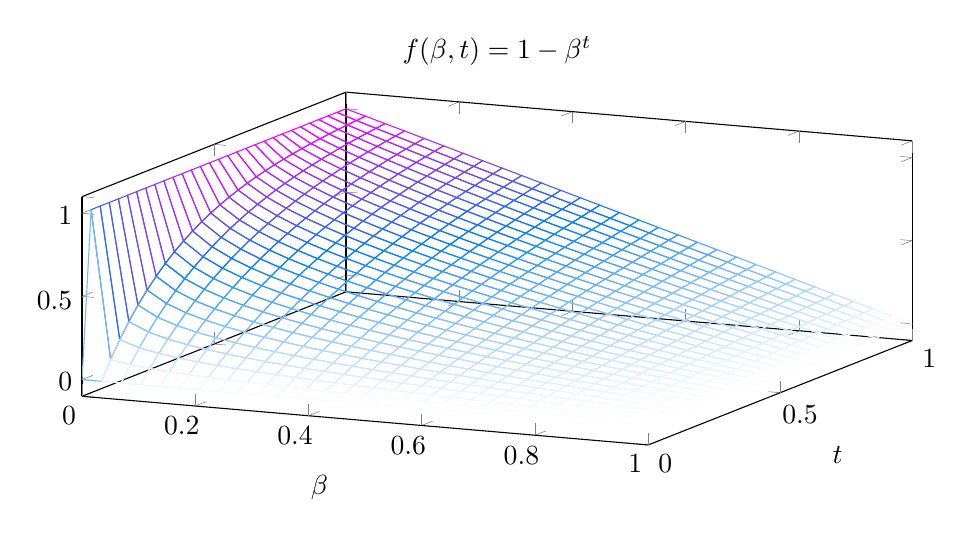
\begin{tikzpicture}
		\begin{axis}
			[
			title={$f(\beta, t) = 1 - \beta^t$},
			%hide axis,
			colormap/cool,
			width = \textwidth,
			height = 0.5 \textwidth,
			xlabel={$\beta$},
			ylabel={$t$}
			] 
			\addplot3[
			mesh,
			samples=30,
			domain=0:1,
			]{1 - x^y};
		\end{axis}
	\end{tikzpicture}
	\caption{Трехмерное изображение корректирующих коэффициентов}
\end{figure}
Данная модель является наиболее простой, однако она обладает возможностью предсказания.
\begin{equation}
	\begin{split}
		v_{t + 1} & = k \cdot y_t + (1 - k) \cdot v_t: \; k \in (0, 1)
	\end{split}
\end{equation}
В данном случае $v_t$ - это предсказанное значение на момент времени $t$. Модель не является устойчивой к наличию сезонности и тренду, однако факт того, что предсказания возможны есть. Значит, эта модель включается в список попадающих в сравнительную таблицу.

		\subsubsection{Auto-regressive Integrated Moving Average}
	Логичным предположением является тот факт, что значения конкретного временного ряда зависят от своих предыдущих значений, как было показано на примере EWMA (\myref{link::ewma}). Обобщая данную мысль, текущее ($t$) значение временного ряда может зависеть от некоторого на $k$ шагов отстающего от него значения ($t - k$). Тогда получается формула вида:
	\begin{equation}
		y_t = \alpha_0 + \sum_{p = 1}^{q} \alpha_p \cdot y_p + \varepsilon_t: \; \varepsilon_t \sim N(0,\sigma^2)
	\end{equation}
	Пока что никаких ограничений на $\alpha_p$ не накладывается. \textbf{Q}: Но что такое переход от $y_t$ элементу ряда к $y_{t - 1}$? \textbf{A}: Это применение некоторого оператора лага (Lag/Backshift) $B: By_t = y_{t - 1}, B^2y_t = y_{t - 2}$ и так далее. \textbf{Q}: Что должен представлять из себя данный оператор? \textbf{A}: 1) Он должен быть линеен, то есть: $B(x_t + k \cdot y_t) = Bx_t + k \cdot By_t = x_{t - 1} + k \cdot y_{t - 1}: k \in \R$. \textbf{Q}: Как грамотно задать данный оператор? \textbf{A}: Представляем ситуацию, в которой необходимо из вектора $Y_n = (y_1, \ldots, y_n)^T$ получить вектор $Y_{n - 1} =  (0, y_1, \ldots, y_{n - 1})^T$, тогда матрица $B: \R^{n \times 1} \to \R^{n \times 1}$ имеет вид.
	\begin{equation}
		\left(\begin{matrix}
			0 & 0 & \cdots & 0\\
			1 & 0 & & 0\\
			\vdots & \ddots & \ddots & \vdots\\
			0 & \cdots & 1 & 0
		\end{matrix}\right) 
		\left(\begin{matrix}
			y_1\\ y_2\\ y_3 \\ \vdots \\ y_n
		\end{matrix}\right) = 
		\left(\begin{matrix}
			0\\ y_1\\ y_2 \\ \vdots \\ y_{n - 1}
		\end{matrix}\right)
	\end{equation}
	Во-первых, она квадратная, во-вторых интересно, что данный оператор является нильпотентным степени $n$. Из этого следует, что a) единственное собственное значение $B$ это $0$ b) $B^n = O$ (нулевая матрица), то есть степень нильпотентности не превосходит $n$. Более подробно в работе \cite{panov_linear_operator}. Но прежде, чем переписать полученную выше сумму в надлежащем виде, вспоминаем о возможной зависимости $y_t$ от предыдущих значений скользящей средней ($\varepsilon_{t - l}$), где $\varepsilon_{t - l}$ - значение, полученное из белого шума \footnote{Белый шум - независимые, взятые из одного распределения величины - часто $N(0,\sigma^2)$.}.
	\begin{equation}
		\begin{split}
			y_t & = \alpha_0 + \sum_{k = 1}^{p} \alpha_k \cdot B^k y_{t} + \sum_{j = 1}^{q} \beta_j \cdot B^j \varepsilon_{t} + \varepsilon_t\\
			\left(1 - \sum_{k = 1}^{p} \alpha_k \cdot B^k\right) y_t & = \alpha_0 + \left(\sum_{j = 1}^{q} \beta_j \cdot B^j\right) \varepsilon_{t}
		\end{split}
	\end{equation}
	При этом $B\alpha_0 = \alpha_0: \alpha_0 \in \R$ по построению. Таким образом, получаем модель авторегрессионной скользящей средней ARMA$(p,q)$. Но по первоначальной предпосылке о стационарности \myref{def::weak_ts_stationarity}, есть желание обобщить модель на случай нестационарных рядов. То есть сделать ее более универсальной. Для этого формально выводим условие стационарности. Выражению $1 - \sum_{k = 1}^{p} \alpha_k B^k$ в соответствие ставим характеристическое уравнение $1 - \sum_{k = 1}^{p} \alpha_k z^k$. Тогда если все корни данного уравнения (в силу Основной теоремы Алгебры, полученный полином над комплексной плоскостью имеет не более, чем $p$ различных корней) $|z_i| > 1$, то данный ряд стационарен. Подробнее для AR(1):
	\begin{equation}
		\begin{split}
			y_t = \alpha \cdot y_{t - 1} + \varepsilon_t \Rightarrow 1 - \alpha \cdot z = 0 \Rightarrow z = \frac{1}{\alpha}\\
			y_{t + 1} - \alpha \cdot y_{t} \approx 0 \Rightarrow \lambda - \alpha = 0 \Rightarrow y_t \approx c \cdot \alpha^t: \; c \in \R 
		\end{split}
	\end{equation}
	Получается, чтобы числовые значения данного ряда не уходили в $\infty$ при $t \to \infty$ необходимо, чтобы в случае AR$(1) \; |z| > 1$, а $|\alpha| < 1$. Аналогично для случаев AR$(p)$. Таким образом, вывод: необходим множитель, который помогал бы последовательности переходить к $d$ - ому порядку интегрирования. \textbf{Q}: Как это сделать? \textbf{A}: $\nabla^1 y_t = y_t - y_{t - 1} = y_t - By_t = (1 - B) y_t, \nabla^2y_t = \nabla^1y_t - \nabla^1 y_{t - 1} = (1 - B) y_t - (1 - B) y_{t - 1} = (1 - B) y_t - (1 - B) By_t = (1 - 2B + B^2) y_t = (1 - B)^2 y_t$ и так далее. Получается, что необходимый множитель: $\nabla^d = (1 - B)^d$. Соответственно формула ARIMA$(p,d,q)$ имеет вид:
	\begin{equation}
		\underbrace{\left(1 - \sum_{k = 1}^{p} \alpha_k \cdot B^k\right) \overbrace{(1 - B)^d}^{\text{I}(d)} y_t}_{\text{AR}(p)} = \overbrace{\alpha_0}^{\text{const}} + \underbrace{\left(\sum_{j = 1}^{q} \beta_j \cdot B^j\right) \varepsilon_{t}}_{\text{MA}(q)}
	\end{equation}
	Получившаяся модель включает в себя авторегрессионную составляющую порядка $p$, скользящую среднюю порядка $q$ и интегрированность порядка $d$. Также стоит отметить, что любой стационарный процесс можно разложить в бесконечный (абсолютно сходящийся) процесс скользящего среднего. Более известен данный факт под названием - разложение Вольда \cite{wold_decomposition}. Для примера предполагаем, что некоторый процесс AR$(1)$ стационарен.
	\begin{equation}
		\begin{split}
			y_t & = \alpha_ 0 + \alpha \cdot y_{t - 1} + \varepsilon_{t}\\
			(1 - \alpha B) \cdot y_t & = \alpha_0 + \varepsilon_{t}\\
			(1 - \alpha B)^{-1}(1 - \alpha B) y_t & = (1 - \alpha B)^{-1} (\alpha_0 + \varepsilon_{t})\\
			y_t & = (1 - \alpha B)^{-1} \cdot \alpha_0 + (1 - \alpha B)^{-1} \cdot \varepsilon_{t}\\
			\text{Но ряд стационарен} \Rightarrow y_t & = \sum_{j = 1}^{\infty} B^j\alpha_0 + \sum_{j = 1}^{\infty} B^j\varepsilon_{t} = \frac{\alpha_0}{1 - \alpha} + \sum_{j = 1}^{\infty} \alpha^j \cdot B^j\varepsilon_{t}
		\end{split}
	\end{equation}
	Более подробно о данной модели написано в \cite{arima}. Процесс обучения (то есть подбора соответствующих коэффициентов модели) происходит посредством применения ММП (Метода Максимального Правдоподобия), максимизирующего вероятность наиболее точно описать входные данные. Глобальная задача, стоящая пред алгоритмом подбора параметров (читать далее - алгоритма обучения) это:
	\begin{equation}
		\sum_{p}^n e_p^2 \to \min_{\alpha \in \R^p, \; \beta \in \R^q}
	\end{equation}
	Где $e_p = y_p - \hat{y}_p$ - остаток (разница между предсказанным и исходным значением). Это очень похоже на Метода Наименьших Квадратов (МНК), только МНК дает аналитическую формулу оценок коэффициентов, а в общем случае это не всегда возможно, поэтому для подобных задач часто применяется ММП. Тут же встает вопрос: \textbf{Q}: Как понять, какая модель лучше описывает данные? \textbf{A}: 1) Критерий Акаике (AIC):
	\begin{equation}
		J_{\text{AIC}} = 2k + n \cdot \ln\left[\frac{1}{n} \sum_{p = 1}^n \left(y_p- \hat{y}_p \right)^2\right]
	\end{equation}
	Где $k$ - количество параметров в обучаемой модели, $n$ - общее количество наблюдений, $(y_p - \hat{y}_p)^2 = e_p^2$ - остаток от регрессии 2) Байесовский информационный критерий (BIC):
	\begin{equation}
	 J_{\text{BIC}} = \frac{1}{n} \sum_{p = 1}^n \left(y_p - \hat{y}_p \right)^2 + \frac{k \hat{\sigma}^2 \ln(n)}{n}
	\end{equation} 
	Где $\hat{\sigma}^2$ - оценка (так как реальное значение неизвестно) дисперсии шума ряда, полученного по формуле $(y - \hat{y})$. \cite{alexandridis2014wavelet} \textbf{Q}: Однако тут появляется еще один вопрос: как человеку понять, какой порядок AR($\cdot$) и MA($\cdot$) должен быть? \textbf{A}: Существует 2 способа, чтобы выяснить это. ACF$(k)$ (Auto Correlation Function) и PACF$(k)$ (Partial Auto Correlation Function). Как видно из названия - это некоторые функции от переменной $k$. \textbf{Q}: Что они характеризуют? \textbf{A}: 1) ACF - основанная на конкретном наборе данных дискретная функция, вычисляемая на основе формулы: 
	\begin{equation}
		\text{ACF}(k) = \hat{\rho}_k = \hat{\text{corr}}(y_t, y_{t - k})
	\end{equation}
	2) PACF - частная автокорреляционная функция. Вычисляется на основе оцененной модели AR$(k)$. Строится график коэффициентов при лагах. В итоге формула функции приобретает вид:
	\begin{equation}
		\text{PACF}(k) = \hat{\alpha}_k
	\end{equation}
	Как было сделано для предыдущей модели, иллюстрируем вышеизложенную теорию на примере. Рассматриваем цены открытия акций компании Apple за 2021 год. Стоит заранее сказать, что прежде, чем обучить модель, проверяем сам ряд на стационарность, то есть - на наличие корней $|z_j| < 1$, что свидетельствует о нестационарности исследуемого ряда.
	\begin{itemize}
		\item В настоящем исследовании проверка стационарности временного ряда проводится посредством применения Аугментированного теста Dickey–Fuller (ADF) \cite{adf_unit_root_test}, а также Kwiatkowski–Phillips–Schmidt–Shin (KPSS) \cite{kpss_unit_root_test}. Для ADF \textbf{H0} - нестационарность (простая незначимость переменной), то есть наличие единичного корня, а для KPSS \textbf{H0} - стационарность ряда.
		\begin{table}[H]
			\centering
			\begin{tabular}{r|cc}
				\toprule
				& ADF & KPSS\\
				\midrule[0.02cm]
				Статистика & $0.017$ & $1.802$\\
				P-val & $0.96$ & $< 0.01$\\
				Критическое значение ($1\%$) & $-3.457$ & $0.739$\\
				Критическое значение ($5\%$) & $-2.873$ & $0.463$\\
				Критическое значение ($10\%$) & $-2.573$ & $0.347$\\
				\midrule[0.02cm]
			\end{tabular}
			\caption{Тестирование исходного ряда на стационарность}
		\end{table}
		Следовательно, ряд не является стационарным. Таким образом, переходим к первым разностям и проводим повторное тестирование.
		\begin{table}[H]
			\centering
			\begin{tabular}{r|cc}
				\toprule
				& ADF & KPSS\\
				\midrule[0.02cm]
				Статистика & $-17.740$ & $0.239$\\
				P-val & $0.00$ & $\gg 0.10$\\
				Критическое значение ($1\%$) & $-3.457$ & $0.739$\\
				Критическое значение ($5\%$) & $-2.873$ & $0.463$\\
				Критическое значение ($10\%$) & $-2.573$ & $0.347$\\
				\midrule[0.02cm]
			\end{tabular}
			\caption{Тестирование первых разностей на стационарность}
		\end{table}
	
		\item Далее строим ACF и PACF, чтобы выяснить порядок авторегрессии и скользящей средней. Делать это уже имеем право, так как полученный процесс является стационарным.
		\begin{figure}[H]
			\centering
			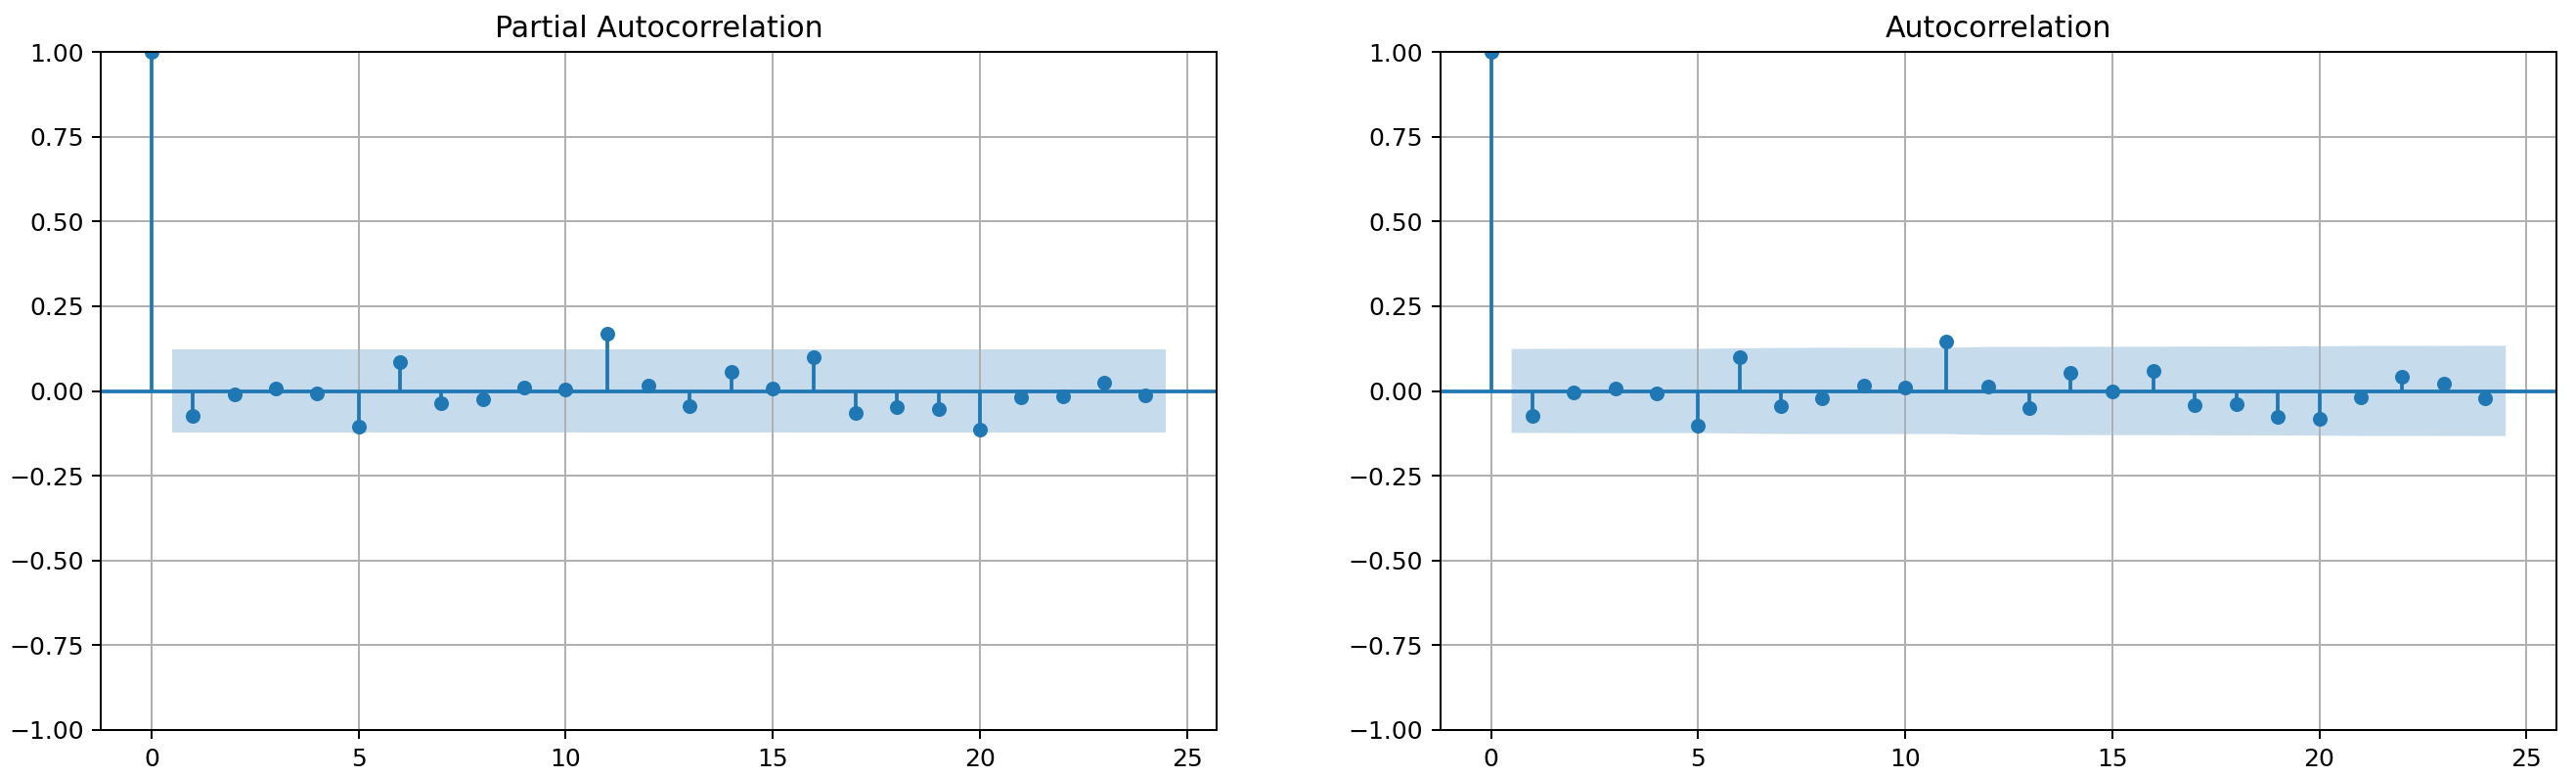
\includegraphics[width=17cm, height=5cm]{arima/initial_acf_pacf.png}
			\caption{ACF и PACF для $\nabla^1y_t$}
		\end{figure}
		В данном случае получаем, что лучшим вариантом модели является случайное блуждание. Модель вида  - пример для Random Walk$(k)$, впервые разработанная Луи Башелье \cite{fama_market_efficiency} в 1900 году в работе, посвященной анализу фондового рынка:
		\begin{equation}
			y_t = \alpha_0 + \sum_{p = 1}^k y_{t - p} + \varepsilon_{t}
		\end{equation}
		То есть формальная запись модели, которую мы оцениваем далее - это ARIMA(0, 1, 0). Так как ни скользящей средней, ни автокорреляции не было выявлено для 1-ой разности.
		
		\item Получаем сводную таблицу о качестве полученной модели:
		\begin{table}[H]
			\centering
			\begin{tabular}{r|ccc}
				\toprule
				Модель & \multicolumn{3}{c}{ARIMA$(0, 1, 0)$}\\
				\midrule[0.02cm]
				Зависимая переменная & \multicolumn{3}{c}{Цена открытия}\\
				Количество наблюдений & \multicolumn{3}{c}{222} \\
				AIC & \multicolumn{3}{c}{$934.71$} \\
				BIC & \multicolumn{3}{c}{$941.56$} \\
				\midrule[0.02cm]
				Тест Ljung-Box (Q) & \multicolumn{2}{c}{$0.04$} & P-val ($0.83$)\\
				Тест Jarque-Bera (JB) & \multicolumn{2}{c}{$6.50$} & P-val ($0.04$)\\
				Тест Heteroskedasticity & \multicolumn{2}{c}{$0.51$} & P-val ($0.00$)\\
				\midrule[0.02cm]
				Константа - $\alpha_0$ & $0.079$ & std (0.135) & P-val (0.557)\\
				Оцененная дисперсия - $\sigma^2$ & $3.949$ & std (0.324) & P-val (0.000)\\
				\midrule[0.02cm]
			\end{tabular}
			\caption{Таблица по оценке иллюстративной модели ARIMA$(0,1,0)$}
		\end{table}
		Тест Ljung-Box \cite{ljung_box_test} - проверка на наличие автокорреляции в остатках. \textbf{H0}: автокорреляции в остатках нет, то есть получен белый шум. Тест Jarque-Bera \cite{jarque_bera_test}- тест на нормальность, где \textbf{H0}: нормальность входных на тест данных. Однако в данном случае присутствует гетероскедастичность, которую можно убрать посредством применения скорректированной ковариационной матрицы HAC \cite{hac_standard_errors}, однако в текущем случае необходим лишь пример модели, а не идеальная ее версия, поэтому оставляем ситуацию с ошибками модели как есть и исследуем остатки регрессии.
		\item В графическом варианте остатки регрессии представляются как некоторый процесс (без тестов не можем сказать, какой именно), а также плотность распределения данного числового ряда.
		\begin{figure}[H]
			\centering
			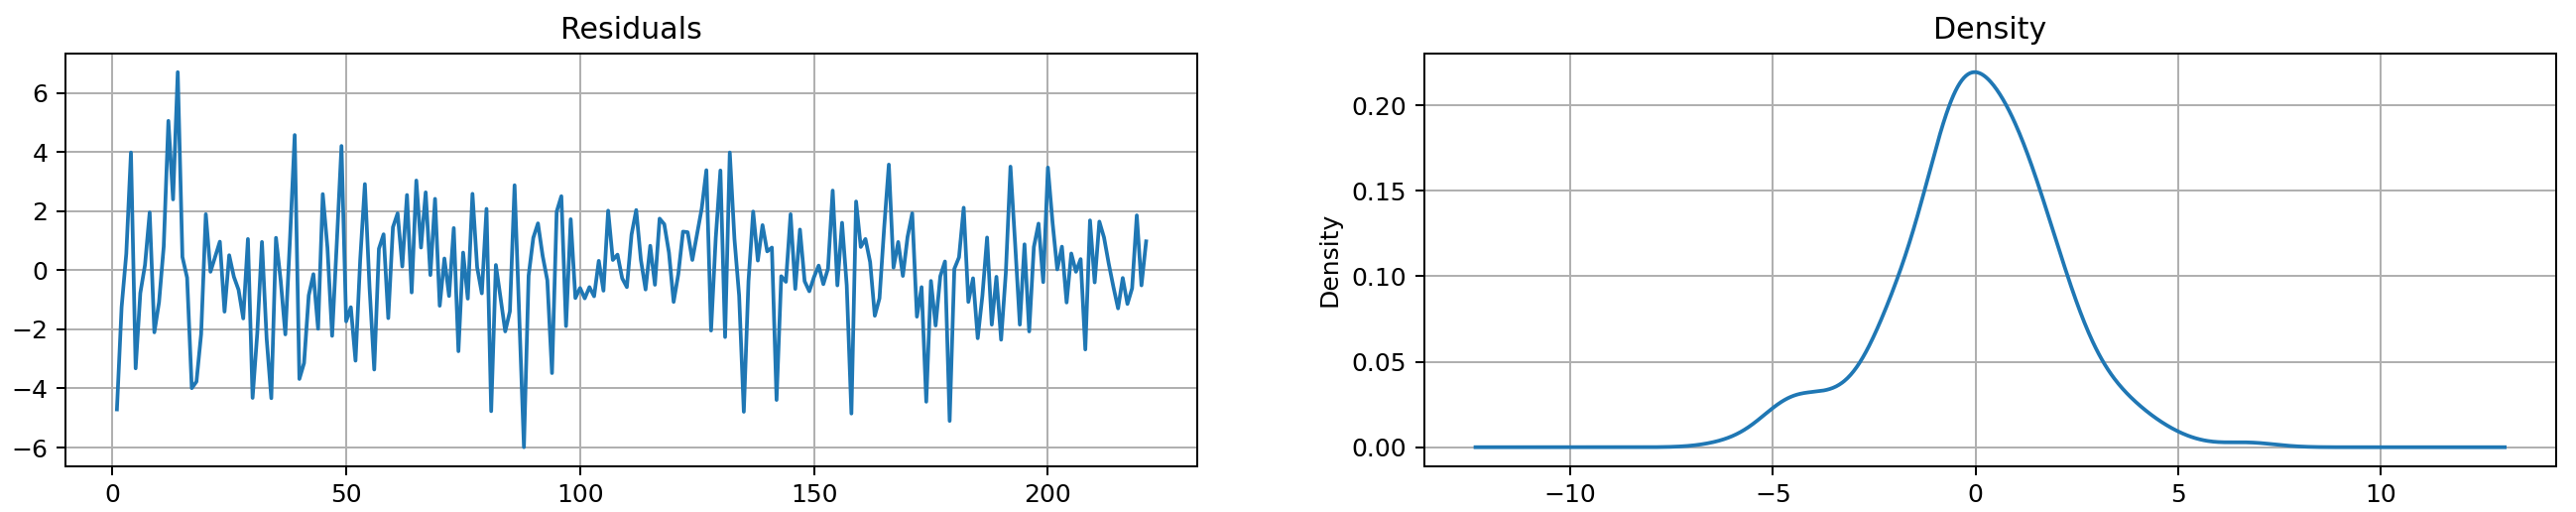
\includegraphics[width=17cm, height=4cm]{arima/residuals_and_density.png}
			\caption{Остатки и распределение остатков моделирования RW}
		\end{figure}
		Исходя из визуального анализа, распределение похоже на нормальное, более того формальные показатели, а именно тесты Ljung-Box и Jarque-Bera, также подтверждают данное предположение. Отсюда вывод, модель подобрана корректно, более ничего необъясненного в данных не осталось. Остался только белый шум. Однако также проверяем: есть ли в остатках модели автокорреляция.
		
		\item Основываясь на графиках ACF и PACF, вывод: автокорреляции в остатках нет.
		\begin{figure}[H]
			\centering
			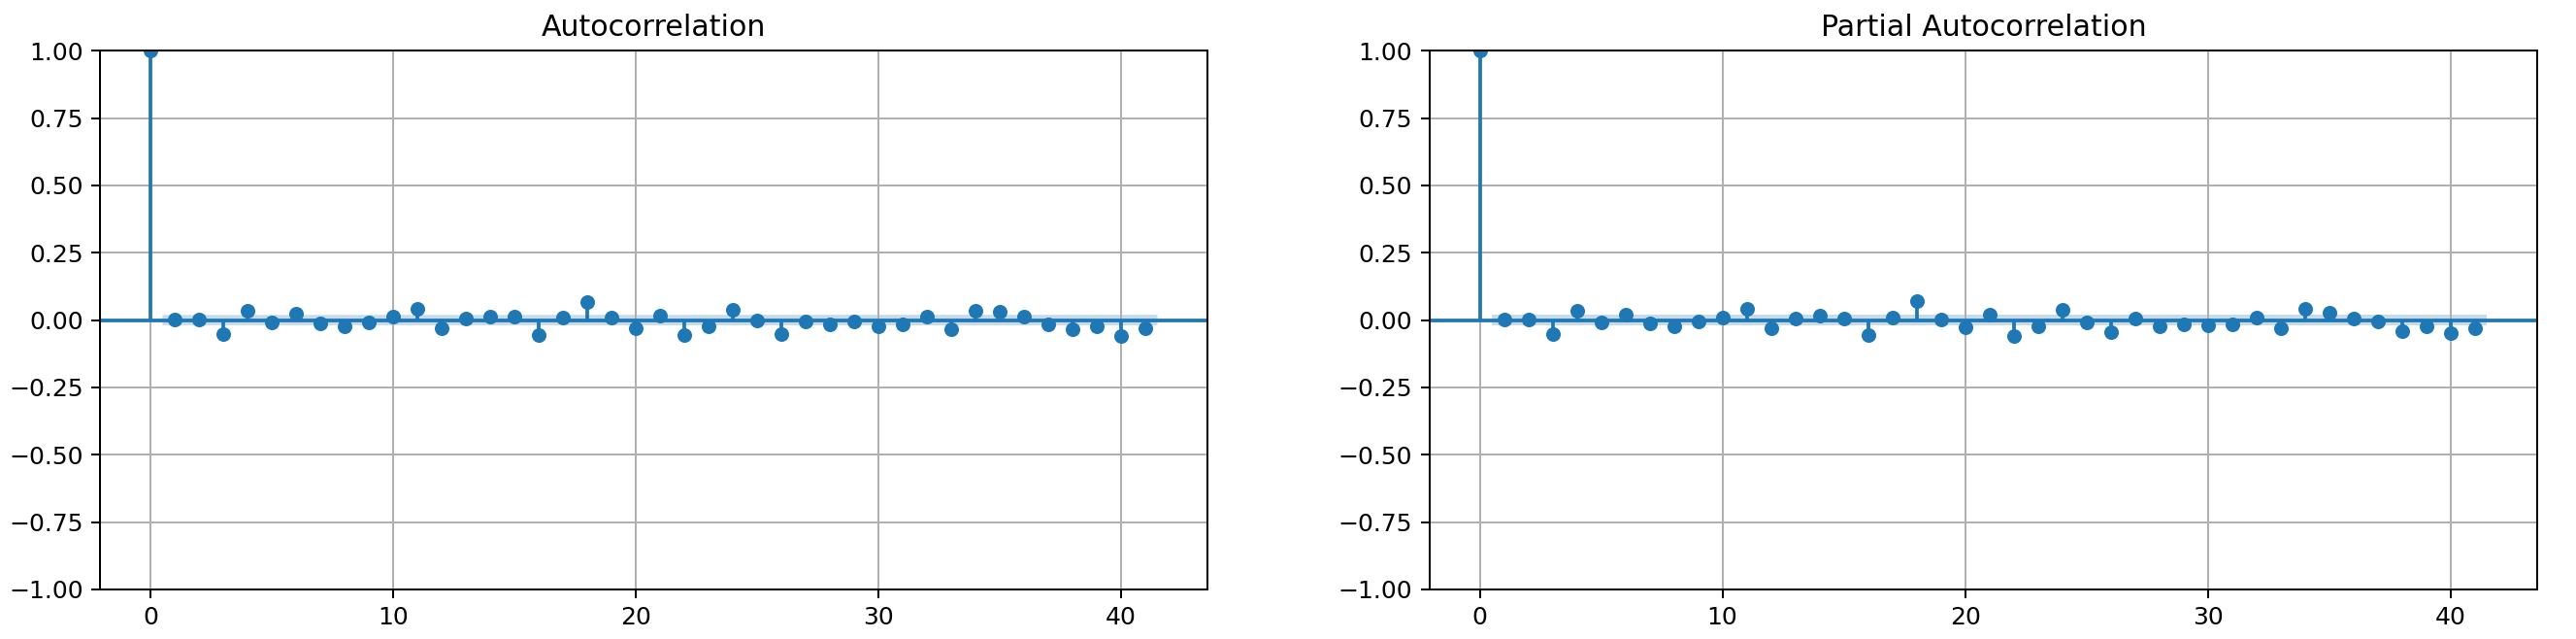
\includegraphics[width=17cm, height=4cm]{arima/residuals_acf_pacf.png}
			\caption{ACF и PACF для остатков моделирования RW}
		\end{figure}
	
		\item Несмотря на информативность уже изображенных графиков, главной ценностью настоящей модели является способность к предсказанию.
		\begin{figure}[H]
			\centering
			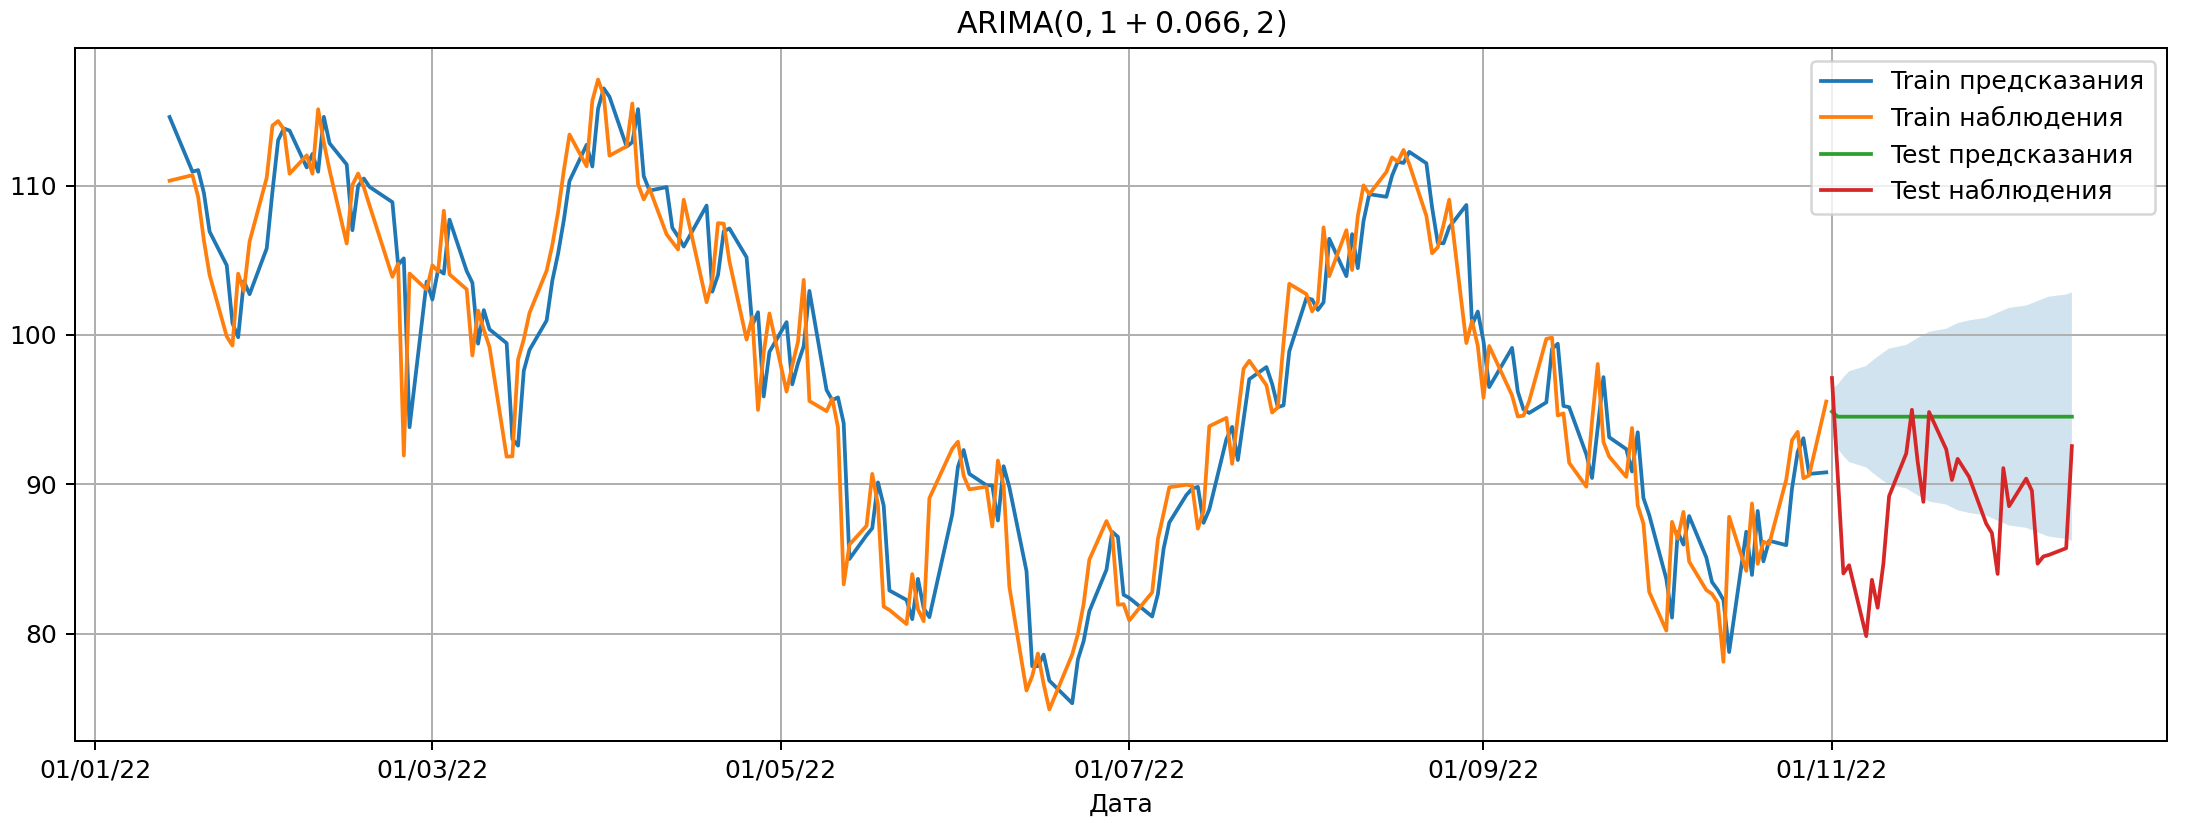
\includegraphics[width=17cm, height=6.25cm]{arima/final_picture.png}
			\caption{Моделирование предсказаний посредством модели RW}
		\end{figure}
	\end{itemize}
	\noindent Здесь синим цветом выделяется доверительный интервал для уровня значимости $5\%$. Причем интересно, что в доверительный интервал почти не попадают реальный значения, что говорит о больших трудностях как для описания данных, так и для предсказания посредством Random Walk. Train/Test - это дробление выборки на обучающие данные (на которых подбираются коэффициенты) и тестовые (на которых проводится проверка адекватности предсказаний модели). Если подобного дробления не проводить, то возможно переобучение, откуда получаем нулевую точность предсказания. Отсюда вывод, что для получения большей точности необходим поиск иного рода моделей. Но, как только что было сказано, с помощью данной модели можно предсказывать последующие значения числовой последовательности, опираясь на исходные показатели временного ряда, поэтому данная модель также включается в список сравнительной таблицы. 
	
		\subsubsection{Generalized Auto-Regressive Conditional Heteroskedasticity}
		\subsubsection{Auto-regressive Fractionally Integrated Moving Average}
Ранее рассматривалась модель ARIMA(p,d,q), принимавшая вид:
\begin{equation}
	\underbrace{\left(1 - \sum_{k = 1}^{p} \alpha_k \cdot B^k\right) \overbrace{(1 - B)^d}^{\text{I}(d)} y_t}_{\text{AR}(p)} = \overbrace{\alpha_0}^{\text{const}} + \underbrace{\left(\sum_{j = 1}^{q} \beta_j \cdot B^j\right) \varepsilon_{t}}_{\text{MA}(q)}
\end{equation}
Для удобства записи, вводим переобозначение $\alpha_p(B) = \left(1 - \sum_{k = 1}^{p} \alpha_k \cdot B^k\right)$, а также $\beta_{q}(B) = \left(\sum_{j = 1}^{q} \beta_j \cdot B^j\right) \varepsilon_{t}$, что преобразует вышенаписанное выражение:
\begin{equation}
	\alpha_p(B) (1 - B)^d y_t = \alpha_0 + \beta_{q}(B) \varepsilon_{t}
\end{equation}
При рассмотрении ARIMA делалось негласное предположение, что $d \in \N$, так как логично, что временные лаги могут быть только целыми и только дискретными. Однако, расширяя данный показатель \cite{fractal_market} на $d \in \R$, получаем процесс, называемый дробно-интегрированным, а само название модели изменяется на ARFIMA, что расшифровывается как авторегрессионная фрактально-интегрированная скользящая средняя. Понятно, что все остальные параметры сохраняются.

ARFIMA$(0, d, 0) \Rightarrow (1 - B)^{d}y_t = \varepsilon_{t} \Rightarrow y_t = (1 - B)^{-d}\varepsilon_t = \sum_{j = 0}^{\infty} h_j\varepsilon_{t - j}$, основываясь на стационарности процесса и разложении Вольда \cite{wold_decomposition}, представляем AR$(1)$ в виде MA$(\infty)$. Далее, воспользовавшись разложением в ряд Тейлора для $(1 - B)^{-d}$, получаем:

\begin{equation}
	\begin{split}
		(1 - B)^{-d} & = 1 + \sum_{p}^{\infty} \frac{(-d)\cdot \ldots \cdot (-d -p + 1)}{p!} (-B)^{p}\\
		(1 - B)^{-d} & = (1 - B)^{-d} = 1 + \sum_{p}^{\infty} \frac{\prod_{i = 1}^{p}(-d - i + 1)}{p!} (-B)^{p}\\
		(1 - B)^{-d} & = 1 + \sum_{p = 1}^{\infty} h_pL^p\\
		h_p & = \frac{\Gamma(p + d)}{\Gamma(d)\Gamma(p + 1)}
	\end{split}
\end{equation}
И из подобного разложения \cite{quantil_2_2007} в случае стационарности следует факт:
\begin{equation} \label{equation::arfima_0_1_0}
	\text{ARFIMA}(0, d, 0): (1 - B)^d y_t = \varepsilon_{t} \Rightarrow y_t = \sum_{j = 0}^{\infty}h_j \varepsilon_{t - j}
\end{equation}
\begin{theorem}[Основные свойства I$(d)$ процесса \cite{hosking_1981}]
	\textbf{Если}: $d < 0.5$, \textbf{то}: процесс стационарен. \textbf{Если}: $d > 0.5$, \textbf{то}: процесс на является стационарным. \textbf{Если}: $d > -0.5$, \textbf{то} разложение \ref{equation::arfima_0_1_0} обратимо. \textbf{Если}: $d \in (-0.5, 0.5)$, \textbf{то}: 1) ковариационная функция: $$y_t: \gamma_k = \frac{\Gamma(1 - 2d) \Gamma(k + d)}{\Gamma(d)\Gamma(1 - d)\Gamma(k + 1 - d)} \sigma^2_{\varepsilon}$$ 2) корреляционная функция при $k \to \infty$ ведет себя как: $$\rho_k \sim \frac{\Gamma(1 - d)}{\Gamma(d)}k^{2d - 1}$$
\end{theorem}
При этом важно заметить, что условия $d \in (-0.5, 0.5)$ всегда можно добиться, применив необходимое количество раз обычное дифференцирование ряда. Все вышеизложенное - преамбула к процессам с долгосрочной памятью.
\begin{definition}[Процесс с длинной памятью]
	\textbf{Если}: $\exists \alpha \in (0, 1), c > 0:$ для ACF верно $\lim\limits_{k \to \infty} \frac{\rho_k}{ck^{-\alpha}} = 1$, \textbf{то}: стационарный процесс называется процессом с длинной памятью.
\end{definition}
Закономерный вопрос: \textbf{Q}: Как эту память обнаружить? \textbf{A}:
\begin{itemize}
	\item Тест Dickey-Fuller и Phillips–Perron (\textbf{H0}: нестационарность) имеют малую мощность, следовательно, они плохо отличают I$(1)$ от I$(d): d < 1$.
	\item KPSS тест (\textbf{H0}: стационарность) состоятелен при стационарных процессах с длинной памятью (I$(d): |d| < 0.5$), но необходимо $\ge 1000$ наблюдений.
	\item Наиболее распространен тест Rescaled Range Statistics (R/S). 
	\item DFA - Detrended Fluctional Analysis (Детрендированный Флуктуационный Анализ). Менее распространен, но применяется.
\end{itemize}
Подводя промежуточный итог, указываем, что в уравнении ARFIMA$(p, d, q)$ отвечает за LM (Long Memory), а что за SM (Short Memory).
\begin{equation}
	\begin{split}
		\alpha_p(B) (1 - B)^d y_t & = \alpha_0 + \beta_{q}(B) \varepsilon_{t}\\
		y_t & = \left(\alpha_p(B) (1 - B)^d\right)^{-1} \left\{\alpha_0 + \beta_{q}(B) \varepsilon_{t}\right\}\\
		y_t & = \underbrace{(1 - B)^{-d}}_{\text{LM}} \underbrace{\alpha_p(B)^{-1} \beta_{q}(B)}_{\text{SM}} \varepsilon_{t}
	\end{split}
\end{equation}
Практическое применения данной модели происходит следующим образом: 1) Оцениваем $d$ 2) Преобразуем ряда 3) Оцениваем $p$ и $q$ при условии, что для нового ряда $d = 0$, то есть ряд стационарен. Исторически одни из первых работ на данную тему были \cite{hosking_1981}, \cite{hurst1951long} применены к изучению в области гидрологии (а точнее - разливам Нила). Главная гипотеза: если в году $t$ засуха, то в году $t + 1$ высока вероятного, что тоже будет засуха. Далее \cite{granger1980introduction} применили данный метод к макроданным. Важно также заметить, что для ARFIMA показатели ACF убывают медленнее, чем для ARIMA, таким образом можно выявить наличие LR (Long Run) памяти визуально. Но более формально это происходить посредством теста R/S, введенного в \cite{hurst1951long}, а примененного к финансовым рядам уже в \cite{mandelbrot1972statistical}. Подробнее R/S рассматривается как отношение значений размаха частичных сумм к стандартному отклонению. \textbf{Q}: Как вычисляется R/S статистика? \textbf{A}:
\begin{enumerate}
	\item Дан ряд $y_1, \ldots, y_{T}$.
	\item Делим исходный ряд на несколько интервалов вида: $n = T$, $n = T / 2$, $n = T / 4$, $\ldots$
	\item Вычисляем статистику:
	\begin{equation}
		\begin{split}
			\text{R/S}_t & = \frac{1}{\hat{\sigma}^2_t} \left(\max_{1 \le k \le t} \left\{\sum_{j = 1}^k (y_j - \overline{y}_t)\right\} - \min_{1 \le k \le t} \left\{\sum_{j = 1}^k (y_j - \overline{y}_t)\right\}\right)\\
			\hat{\sigma}^2_t & = \frac{1}{t} \sum_{j = 1}^t (y_t - \overline{y}_t)^2 \;\;\; \overline{y}_t = \frac{1}{t} \sum_{j = 1}^t y_j
		\end{split}		
	\end{equation}
	\item Предполагаем для R/S статистика, что она увеличивается пропорционально корню из временного промежутка. Тогда:
	\begin{equation}
		\begin{split}
			\text{R/S}_t & \approx \frac{\sum_{j = 1}^t R_j}{\sum_{j = 1}^t S_j} \approx (c \cdot n)^H: n \to \infty\\
			\log\left(\text{R/S}_t\right) & \approx \hat{c} + \hat{H} \log(\hat{n})
		\end{split}
	\end{equation}
	Где $R_n$ - размах, $S_n$ - стандартное отклонение, $c$ - константа, $H$ - показатель Херста (часто называется экспонента Херста).
\end{enumerate}
Выводы: 1) \textbf{Если}: $H > 0.5$ и значима, \textbf{то}: процесс называется персистентным, то есть следующие друг за другом приращения процесса имеют тенденцию сохранять знак и имеют положительную автокорреляцию. \textbf{Если}: $H = 0.5$ и значима, \textbf{то}: тенденции не выражено (например, белый шум). \textbf{Если}: $H < 0.5$, \textbf{то}: процесс антиперсистентен и имеет отрицательную автокорреляцию (любая тенденция стремится смениться на противоположную). Таким образом, получаем алгоритм действий:
\begin{enumerate}
	\item Рисуем ACF для исходного процесса. Если ACF убывает гиперболически, то возможно, что процесс дробно-интегрированный.
	\item Доводим ряд до стационарности путем классического дифференцирования.
	\item Вычисляем константу Херста.
	\item Переходим от ARIMA к ARFIMA.
\end{enumerate}
Однако у данного подхода есть свои недостатки: 1) Чувствительность к SR зависимости 2) Чувствительность к гетероскедастичности. Существует решение, предложенное Andrew Lo \cite{andrew1991longterm}. Идея решения - преобразование $\sigma^2$.
\begin{equation}
	\begin{split}
		Q_t \equiv \text{R/S}_t & = \frac{1}{\hat{\sigma}^2_t(q)} \left(\max_{1 \le k \le t} \left\{\sum_{j = 1}^k (y_j - \overline{y}_t)\right\} - \min_{1 \le k \le t} \left\{\sum_{j = 1}^k (y_j - \overline{y}_t)\right\}\right)\\
		\hat{\sigma}^2_t(q) & = \hat{\sigma}^2_t + 2 \sum_{j = 1}^q \omega_j(q) \hat{\gamma}_{jt}\\
		\omega_j(q) & = 1 - \frac{j}{q + 1}: \; q < t\\
		\hat{\gamma}_{jt} & = \frac{1}{t} \sum_{i = j + 1}^t (y_i - \overline{y}_t)(y_{i - j} - \overline{y}_t)
	\end{split}
\end{equation}
Где $\hat{\sigma}^2_t$ и $\hat{\gamma}_j$ - дисперсия и автоковариация для $y$. Тестирование наличия LR памяти имеет \textbf{H0}: SR память.Критические значения для данной статистики другие, а именно:
\begin{table}[H]
	\centering
	\begin{tabular}{c|cc}
		\toprule
		$\alpha$ & Левый край & Правый край\\
		\midrule[0.02cm]
		1\% & $[0.721$ & $2.098]$\\
		5\% & $[0.809$ & $1.862]$\\
		10\% & $[0.861$ & $1.747]$\\
		\midrule[0.02cm]
	\end{tabular}
	\caption{Критические значения для модифицированного R/S}
\end{table}
\noindent Другим способом оценки показателя $H$ является DFA, работающий по принципу: "Убирай все, что кажется трендом и анализируй остаток". Формальный алгоритм оценки имеет следующий вид \cite{garafutdinov2021research}:
\begin{enumerate}
	\item Дан ряд $y_t: t = \overline{1, T}$.
	\item Вычисляем $y^{\text{cum}}_t = \sum_{i = 1}^t (y_i - \overline{y}_t)$.
	\item Разбиваем куммулятивный ряд на $N$ сегментов длины $\delta$.
	\item Для каждого сегмента вычисляем:
	\begin{equation}
		F_i(\delta) = \sqrt{\frac{1}{\delta} \sum_{t = i \cdot \delta + 1}^{(i + 1) \cdot \delta} \left(y_t^{\text{cum}} - y^{\text{trend}}_t \right)^2}: i = \overline{0, N - 1}
	\end{equation}
	$F_i(\delta)$ и есть флуктуационная функция, а $y^{\text{trend}}_t$ - значение в точке $t$ функции локального линейного тренда, аппроксимирующего динамику данного ряда.
	\item Полученные значения далее усредняются:
	\begin{equation}
		\overline{F(\delta)} = \frac{1}{N}\sum_{j = 1}^N F_i(\delta)
	\end{equation}
	\item Все расчеты проводятся для нескольких $\delta$.
	\item Далее оценивается линейная регрессия:
	\begin{equation}
		\ln(\overline{F(\delta)}) = \alpha \ln(\delta) + b: \alpha, b \in \R
	\end{equation}
	\item В итоге экспонента Херста равна:
	\begin{equation}
		H = \left\{\begin{array}{rl}
			\alpha & \text{, } y_t - \text{стационарен}\\
			\alpha - 1 & \text{, } y_t - \text{нестационарен}\\
		\end{array}\right.
	\end{equation}
\end{enumerate}

\noindent Далее оцениваем ARFIMA на реальных данных. Аналогично всем моделям раньше, используем в качестве образца цена открытия акций Apple за 2021.\\

\#TODO: Эксперимент.
		\subsubsection{Fractionally Integrated GARCH}
		\subsubsection{Singular Spectrum Analysis}
До этого момента все рассмотренные модели использовали в своей основе идею о стационарности, представленную в определении (\myref{def::weak_ts_stationarity}) и (\myref{def::strong_ts_stationarity}). Теперь же рассматриваем иной подход, основанный на отсутствии предпосылок относительно исходных данных. То есть теперь имеющийся набор значений воспринимается как сигнал, характеризующий объект на некотором промежутке времени. Иными словами, нет необходимости предполагать как распределены данные или думать, что все имеющиеся значения - реализации набора случайных величин. Пользуясь определением (\myref{def::signal_stationarity}), рассматриваем следующее преобразование исходного ряда.

Исследуемый метод основывается на сингулярном разложении матрицы траекторий (она же матрица Ханкеля), отборе необходимого количества главных компонент (в методе Principal Component Analysis \cite{abdi2010pca}) и последующей реконструкции (аппроксимации) исходного ряда. Название метода за рубежом - Singular Spectrum Analysis (SSA), в России - Гусеница \cite{catarpillar_ssa}. То есть сам алгоритм SSA имеет 2 этапа: разложение и реконструкция. Рассматриваем каждый их них отдельно.

Пусть дан исходный ряд вида  ${Y = (y_0, ..., y_{N - 1})}$, преобразуем его в матрицу траекторий (Ханкелиан). Для этого выполняем операцию:
\begin{equation} \label{eq::hankelisation}
	Y \rightarrow X \in \R^{L, K}: L \in [2, \lfloor N / 2 \rfloor], K = N - L + 1
\end{equation}
\noindent Основываясь на методе Singular Vector Decomposition (SVD) \cite{martin2012svd}, получаем декомпозицию:
\begin{equation}
	X = \underbrace{U}_{L \times L} \underbrace{\Sigma}_{L \times K} \underbrace{V^*}_{K \times K}
\end{equation}
Где ${d - \textbf{ранг}(X)}$. Для ортонормальной $V \in \R^{K,K} \Rightarrow V^{-1} = V^T$ и второй случай: ${V \in \mathbb{C}^{K, K} \Rightarrow V^* = \left(\overline{V}\right)^T}$ - Эрмитово сопряжение. Столбцы ${U}$ образуют ортонормированный базис в пространстве столбцов X, а столбцы ${V}$ - в пространстве строк X. ${\Sigma}$, в свою очередь, <<диагональная>> матрица, составленная из сингулярных чисел ${XX^T}$ и ${X^TX}$, $T$ - операция транспонирования. Далее замечаем, что разложение  $X$ можно представить в виде суммы элементарных матриц:
\begin{equation} \label{eq::ssa_decomposition}
	X = \sum_{j = 1}^{d} \sigma_j U_j V_j^* = \sum_{j = 1}^{d} \sigma_j \overbrace{U_j}^{L \times 1} \overbrace{V_j^*}^{1 \times K} = \sum_{j = 1}^{d} X_j = \sum_{s \in S} X_s + \sum_{t \in T} X_t + \sum_{o \in O} X_o
\end{equation}
Где $|S| + |T| + |O| = d$, при этом интересно, что $\sigma_j = \sqrt{\lambda_j}$ - где $\lambda_j$ - собственное значение матрицы X, когда она квадратная. Далее, $(\sigma_j, U_j, V_j)$ - вклад $j$-ой собственной тройки в матрицу X. Иначе: как много информации об $X$, где $X$ - Ханкелиан от исходного временного ряда, содержит $j$-я элементарная матрица. $s \in S$ - компоненты сезонности, $t \in T$ - компоненты тренда, $o \in O$ - все остальные компоненты. Важно, что в настоящем исследовании ранее было оговорено, что сезонность в финансовых рядах подобного вида отсутствует, то есть признается наличие только тренда и шума. То есть даже если сезонность присутствует, то ее компоненты относятся к шуму. На данном этапе говорим, что первый пункт плана (декомпозиция) выполнен. Приступаем ко второму - реконструкции.

Очевидно, если сложить все элементарные матрицы, то по (\ref{eq::ssa_decomposition}) получаем исходную матрицу $X$, но это не исходный ряд. Таким образом, встает вопрос \textbf{Q}:  Как из Ханкелиана получить ряд? \textbf{A}: Для этого используется оператор Деханкелизации. 
\begin{equation}
	\begin{split}
		\hat{H}: \; & L\times K \rightarrow N\\
		\tilde{X_j} & = \hat{H}X_j - \text{ элементы на побочной диагонали $\approx$ равны.}\\
		\tilde{X_j} & \stackrel{\text{avg}}{\rightarrow} \tilde{Y_j} - \text{ восстановленный $Y$ через усреднение.}
	\end{split}
\end{equation}
Для получения некоторого ряда из элементарной матрицы применяется также оператор усреднения по побочной диагонали, задаваемый формулой:
\begin{equation} \label{eq::dehankelisation}
	\tilde{x}_{m,n} = 
	\left\{\begin{array}{ll}
		\displaystyle
		\frac{1}{s + 1} \sum_{l = 0}^s x_{l, s - l} & \text{, } 0 \le s \le L - 1\\
		\displaystyle
		\frac{1}{L - 1} \sum_{l = 0}^{L - 1} x_{l, s - l} & \text{, } L \le s \le K - 1\\
		\displaystyle
		\frac{1}{K + L - S - 1} \sum_{l = s - K + 1}^L x_{l, s- l} & \text{, } K \le s \le K + L - 2
	\end{array}\right.
\end{equation}
\noindent Где $s = m + n$. Также интересно, что  $\hat{H}$ является линейным. Доказываем это:
\begin{lemma}
	Оператор деханкелизации $\hat{H}: L \times K \to N$ является линейным.
\end{lemma}
\begin{proof}
	Для того, чтобы оператор являлся линейным необходимо выполнение свойств: 1) $\hat{H}(A + B) = \hat{H}A + \hat{H}B$, где $A, B \in \mathbb{X} \subset \R^{L \times K}$, для которого определен оператор $\hat{H}$ 2) $\hat{H}(\alpha A) = \alpha \hat{H}A$, где $\alpha \in \R$. Рассматриваем по-порядку:
	\begin{enumerate}
		\item Пусть изначально есть 2 ряда $a$ и $b$ длины $N$. После этого они переводятся в матрицу траекторий путем ханкелизации (\ref{eq::hankelisation}). Получаем 2 матрицы $A, B \in \R^{L \times K}$, где на побочной диагонали стоят одинаковые элементы. При этом $L$ не обязательно равно $K$, в таком случае получаем название не <<побочная диагональ>>, а <<антидиагонали>>. После этого $C = A + B$, соответственно на антидиагоналях $C$ стоят одинаковые элементы, таким образом $\hat{H}C = a + b$, но по определению ханкелизации - переходу к матрице траекторий - получаем, что $\hat{H}C = \hat{H}A + \hat{H}B$.
		\item Теперь рассматриваем $\alpha A: \alpha \in R, A \in \R^{L \times K}$. Получаем, что каждый элемент матрицы умножается на $\alpha$, однако, как было сказано в (\ref{eq::dehankelisation}), диагональные элементы усредняются. Таким образом, получаем, что каждый элемент исходного ряда умножается на $\alpha$, но если $\alpha$ везде одинаковое, то просто выносим его из данного вектора, что равносильно $\hat{H}(\alpha A) = \alpha \hat{H}A$.
	\end{enumerate}
\end{proof}

\noindent Из вышедоказанной леммы следует, что:
\begin{equation}
	X = \hat{H}X = \hat{H} \left(\sum_{j = 1}^{d} \sigma_j U_j V_j^*\right) = \sum_{j = 1}^{d} \hat{H}X_j = \sum_{j = 1}^{d} \tilde{X}_j
\end{equation}
\noindent Теперь определяемся с тем, какие именно компоненты (элементарные матрицы) необходимо взять, чтобы получился сигнал, лишенный шума. Теперь главной задачей является избавление от шума, чтобы в итоге восстановленный ряд имел вид:
\begin{equation}
	\hat{Y} = \hat{H} \sum_{t \in T} \sigma_t U_t V^*_t = \sum_{t \in T} \hat{H}X_j 
\end{equation}
\noindent Где $Y - \hat{Y}$, по предположению, шум. \textbf{Q}: Как понять, какие компоненты выбрать? \textbf{A}: корреляционная матрица, построенная на основе взвешенного скалярного произведения. \textbf{Q}: Откуда брать веса? Какими они должны быть? \textbf{A}: В качестве весов используем количество раз, которое каждое число встречается на побочной диагонали элементарной матрицы траекторий. Сам вес задаем формулой:
\begin{equation}
	w_k = \left\{\begin{array}{ll}
		k + 1 & \text{, } 0 \le k \le L - 1\\
		L & \text{, } L \le k \le K - 1\\
		N - k & \text{, } K \le k \le N - 1
	\end{array}\right.
\end{equation}
На основе этих весов строим корреляционную матрицу:
\begin{equation}
	W_{corr} = \left\{ w_{i, j} = \frac{\left(\tilde{Y}_j, \tilde{Y}_i\right)_w}{\lVert \tilde{Y}_i \rVert_w \lVert \tilde{Y}_j \rVert_w} \right\}_{i, j = 0}^{N - 1}: \left(\tilde{Y}_j, \tilde{Y}_i\right)_w = \sum_{k = 0}^{N - 1} w_k \cdot \tilde{y}_{i, k} \cdot \tilde{y}_{j, k}
\end{equation}
$w_{i, j} \rightarrow 1$ если $\tilde{Y}_i$ и $\tilde{Y}_j$ близки, иначе $w_{i, j} \rightarrow 0$. Пороговое значения для группировки задается как гиперпараметр, что делает данный метод менее универсальным, но позволяет решить вопрос выбора компонент. 

Предсказания последующих значений исследуемого ряда происходит по следующему алгоритму \cite{catarpillar_ssa}:
Важно: ${U_j}$ - $j$ столбцы $U$, а ${\tilde{y}_t}$ - реконструированный ряд без компоненты шума.
\begin{enumerate}
	\item Подсчитываем ${r = \lvert \left\{\sigma_j: \sigma_j > 0 \right\} \rvert}$.
	\item Берем ${\left\{ \underline{U}_{j, k} : 1 \le j \le r, 1 \le k < L \right\}: U}$ -  матрица с ортонормированными столбцами.
	\item Берем ${\left\{\pi_j : \pi_j = U_{j, L}: j = \overline{1, r}\right\}}$ - ${\pi_j}$ - последний элемент каждого из $r$ столбца матрицы $U$.
	\item Вычисляем $\nu^2 = \sum_{j = 1}^r \pi_j^2$.
	\item Вычисляем вектор коэффициентов ${R = \left(a_{L - 1}, \ldots, a_{1}\right)^T = \frac{1}{1 - \nu^2} \sum_{j = 1}^r \pi_j \underline{U}_j}: \underline{U}_j \in \R^{L-1 \times 1}$
	\item Для прогнозирования используется формула:
	\begin{equation}
		y_t = 
		\left\{\begin{array}{ll}
			\displaystyle
			\tilde{y}_t & \text{, } t = \overline{1, N}\\
			\displaystyle
			\sum_{j = 1}^{L - 1}a_j y_{t - j} & \text{, } t = \overline{N+1, N + h}
		\end{array}\right.
	\end{equation}
	\noindent Для интереса: более подробно о деталях предсказания временных рядов методом SSA в \cite{catarpillar_ssa}.
\end{enumerate}

Второй этап (реконструкция) тоже закончен, однако остается два вопроса: 1) Чему изначально должна равняться переменная $L$, отвечающая за количество компонент, на которые производится разбиение? 2) Как наиболее точно разделить все компоненты по группам, максимальной удалив шум? Отвечаем на данные вопросы последовательно: 1) Существуют решения и предложения по данному вопросу \cite{catarpillar_ssa}, \cite{wang2015selection}, однако до конца данный вопрос разрешается только, исходя их задачи, к которой применяется SSA 2) Существует еще больше методов, позволяющих произвести подобное разбиение \cite{catarpillar_ssa}, \cite{kuang2020efficient}, \cite{lin2019grouping}, \cite{lin2016grouping}, однако аналогично предыдущему вопросу на этот тоже нет точного ответа. Для примера в настоящем исследовании проводится изучение и реализация алгоритма, описанного в \cite{kuang2020efficient}. Также интересно, что алгоритм предсказания является итерационным, то есть для получения одного нового значения необходимо полностью повторить все действия, что по аналогии сравнимо с <<гусеницей>>.

Главная задача, стоящая перед авторами \cite{kuang2020efficient}, - это предложить устойчивый к входным данным  и эффективный алгоритм <<очищения>> исходного сигнала посредством применения многоразового SSA. Ключевое отличие предложенного метода от непосредственно ручного очищения сигнала - универсальность и отсутствие гиперпараметров. В исходном SSA алгоритме данных параметров целых 2: $L$ - количество компонент и $M$ - количество групп, на которые производится разбиение полученных компонент. Таким образом, встает вопрос о необходимости автоматизации выбора данных параметров или о предложении алгоритма с совершенно иным подходом, лежащим в основе группировки компонент.

Идея метода в итеративном разбиении исходного сигнала посредством классического SSA на $L_1$ компонент и дальнейшей группировке на <<шум>> и не <<шум>>.  То есть сигнал, признанный лишенным шума на шаге  $i$, на шаге $i + 1$ принимается за сигнал с шумом. Таким образом, алгоритм повторяется далее и далее до тех пор, пока не выполняется критерий останова. В случае отсутствия оного, исход алгоритма упирается в количество заданных итераций: возможна ситуация, когда важная компонента, не относящаяся к шуму, из-за большого количество шагов алгоритма классифицируется как шумовая. Следовательно, часть важной информации о сигнале теряется. Если же количество итераций слишком мало, то сигнал все равно остается зашумленным.

На $i$-й итерации сигнал дробится на $L_1$ компонент, а далее оператором $G$ - Grouping разбивается на группы: сигнал и шум. На $i + 1$-й итерации сигнал, признанный лишенным шума на $i$-м этапе опять делится на $L_1$ элементов, после чего все полученные элементы распределяются оператором $G$ на 2 группы. Таким образом, задав $ds_m$ (от denoised signal) - сигнал без шума на итерации $m$, а $o_m$ (от other) - компонента шума на итерации $m$, получаем соотношение:
\begin{equation}
	ds_m = ds_{m + 1} + o_{m + 1}
\end{equation}
Где $m = \overline{1, M}$, $M \in \N$ - общее количество итераций алгоритма. Более того, согласно \cite{kuang2020efficient}, исходный сигнал полноценно восстанавливается в виде:
\begin{equation}
	x = ds_m + n_m = ds_m + \sum_{i = 1}^m o_m
\end{equation}
$n_m$ - накопленные за $m$ шагов компоненты шума. Таким образом, финальный алгоритм по очистке сигнала от шума, представленный в \cite{kuang2020efficient}, имеет вид (aлг.~\ref{alg::signal_denoising_ssa}). 

Алгоритм весьма лаконичен и прост. Ключевая его особенность - критерий останова в строке 6, в которой сказано следующее: <<Вычисляем разницу между сигналами в момент $m$ и $m - 1$, но при этом смотрим, чтобы итоговое значения было больше $0$, что гарантирует сохранение тренда>>. Однако при этом остается один гиперпараметр $M$, задающий общее количество итераций. Он необходим для данного алгоритма, так как без него процесс дробления продолжается бесконечно. Таким образом, наличие цикла for гарантирует конечность алгоритма как такового.
\begin{algorithm}[H]
	\caption{Очистка исходного сигнала от шума} \label{alg::signal_denoising_ssa}
	\begin{algorithmic}[1]
		\Require $x \in R^N$ - исходный сигнал.
		\Require $L_1 = 2$ - размер окна.
		\State Вычисляем: $ds_1$ и $n_1 = o_1$ через $SSA(L_1, G)$
		\State Вычисляем: скалярное произведение $\langle ds_1, n_1 \rangle = \sum_{j = 1}^N ds_{1j} \cdot n_{1j}$
		\For{$m = \overline{1, M}$}
			\State Вычисляем: $ds_m$ и $n_m = \sum_{j = 1}^m o_j$ через $SSA(L_1, G)(ds_{m - 1})$
			\State Вычисляем: скалярное произведение $\langle ds_m, n_m \rangle = \sum_{j = 1}^N ds_{mj} \cdot n_{mj}$
			\If{$\langle ds_m, n_m \rangle - \langle ds_{m - 1}, n_{m - 1} \rangle > 0$}
				\State \textbf{break}
			\EndIf
		\EndFor
		\State \Return оптимальное количество итераций: $m_{opt} = m - 1$, где $m$ - значение, на котором завершился цикл.
		\State \Return сигнал $ds_{m - 1}$, очищенный от шума.
	\end{algorithmic}
\end{algorithm}
\noindent Теперь, основываясь на вышеизложенной теории, рассматриваем практические применение как самого SSA алгоритма, включающего декомпозицию, реконструкцию и предсказание, так и Multistage SSA (MSSA).

\subsubsubsection{Пример: SSA}
\\\\
В качестве искусственных данных исследуем результат применения закона:
\begin{equation} \label{link::illustr_func}
	f(x) = \frac{1}{4}x^2 + \sin(5x) + \cos(x) \cdot \varepsilon: \varepsilon \sim N(0, I_n)
\end{equation}
Где $f: \R^n \to \R^{n}$, а $\varepsilon$ - вектор белого шума, $I_n$ - единичная матрица размера $n \times n$. Графически результат работы данной функции имеет вид:
\begin{figure}[H]
	\centering
	\begin{tikzpicture}
		\begin{axis}[
			grid = both,
			legend pos = north west,
			minor tick num = 1,
			major grid style = {lightgray},
			minor grid style = {lightgray!25},
			%title= {},
			width = \textwidth,
			height = 0.45 \textwidth,
			xmin=-5, xmax=5,
			ymin=-4, ymax=7.5,
			line width=0.3mm
			]
			
			\addplot[opacity = 0.25, color = blue] table [
			x=x, 
			y=y, 
			col sep=comma,
			mark={},
			] {./source/source_csv/Illustration data/ssa/data_to_denoise.csv};
			
			\addplot[domain = -5:5,
			samples = 300,
			color = teal,
			smooth,
			line width = 0.05cm,] {sin(deg(5 * x)) + 1 / 4 * (x^2)};
			
			\legend{$f(x)$, $f(x)$ без шума};
		\end{axis}
	\end{tikzpicture}
	\caption{Построение $f(x)$. см. выражение (\ref{link::illustr_func})}
\end{figure}
В настоящем сигнале присутствуют как трендовая $1/4 \cdot x^2$ и сезонная $\sin(5x)$ составляющие, так и необычный (гетероскедастичный: с различающийся дисперсией) шум $\cos(x) \cdot \varepsilon$. Таким образом, можно уверенно пытаться применить SSA для расщепления данного сигнала на составляющие.

Пусть для начала $L = 20$, то есть количество компонент, на которые проводится расщепление составляет $20$ штук. Для предсказаний используем последние $100$ значений из $2'000$. Тогда общий вид разложения с учетом исходных выглядит следующим образом:
\begin{figure}[H]
	\centering
	\begin{tikzpicture}
		\begin{axis}[
			grid = both,
			legend pos = south east,
			minor tick num = 1,
			major grid style = {lightgray},
			minor grid style = {lightgray!25},
			%title= {},
			width = \textwidth,
			height = 0.45 \textwidth,
			xmin=-5, xmax=5,
			ymin=-4, ymax=7.5,
			line width=0.3mm
			]
			
			\addplot[opacity= 0.25] table [
			x=x, 
			y=y, 
			col sep=comma,
			mark={}
			] {./source/source_csv/Illustration data/ssa/data_to_denoise.csv};
			
			\addplot[domain = -5:5,
			samples = 300,
			color = green,
			smooth,
			line width = 0.05cm] {sin(deg(5 * x)) + 1 / 4 * (x^2)};
			
			\addplot[line width = 0.05cm, color= blue] table [
			x=x, 
			y=y1, 
			col sep=comma,
			mark={},
			] {./source/source_csv/Illustration data/ssa/components.csv};
			
			\addplot table [
			x=x, 
			y=y2, 
			col sep=comma,
			mark={},
			] {./source/source_csv/Illustration data/ssa/components.csv};
			
			\addplot table [
			x=x, 
			y=y3, 
			col sep=comma,
			mark={},
			] {./source/source_csv/Illustration data/ssa/components.csv};
			
			\addplot table [
			x=x, 
			y=y4, 
			col sep=comma,
			mark={},
			] {./source/source_csv/Illustration data/ssa/components.csv};
			
			\addplot table [
			x=x, 
			y=y5, 
			col sep=comma,
			mark={},
			] {./source/source_csv/Illustration data/ssa/components.csv};
			
			\addplot table [
			x=x, 
			y=y6, 
			col sep=comma,
			mark={},
			] {./source/source_csv/Illustration data/ssa/components.csv};
			
			\legend{$f(x)$, $f(x)$ без шума, Компонента 1};
		\end{axis}
	\end{tikzpicture}
	\caption{Декомпозиция $f(x)$. см. выражение (\ref{link::illustr_func})} \label{fig::illustr_decomposition}
\end{figure}
\noindent Большинство компонент показывают себя как гетероскедастичный шум и лишь только одна компонента, соответствующая большему сингулярному числу матрицы Ханкеля от исходного ряда, обозначенная на графике, являет собой нечто похожее на тренд.
\begin{figure}[H]
	\centering
	\begin{tikzpicture}
		\begin{axis}[
			grid = both,
			legend pos = north west,
			minor tick num = 1,
			major grid style = {lightgray},
			minor grid style = {lightgray!25},
			%title= {},
			width = \textwidth,
			height = 0.45 \textwidth,
			xmin=1, xmax=20,
			ymin=0, ymax=0.025,
			line width=0.3mm
			]
			
			\addplot table [
			x=x, 
			y=each, 
			col sep=comma,
			%mark={},
			] {./source/source_csv/Illustration data/ssa/contribution.csv};
			
			\legend{Каждая компонента};
		\end{axis}
	\end{tikzpicture}
	\caption{<<Информативность>> каждой компоненты}
\end{figure}

\begin{figure}[H]
	\centering
	\begin{tikzpicture}
		\begin{axis}[
			grid = both,
			legend pos = north west,
			minor tick num = 1,
			major grid style = {lightgray},
			minor grid style = {lightgray!25},
			%title= {},
			width = \textwidth,
			height = 0.45 \textwidth,
			xmin=1, xmax=20,
			ymin=0.9, ymax=1,
			line width=0.3mm
			]
			
			\addplot[color= red] table [
			x=x, 
			y=cumsum, 
			col sep=comma,
			%mark={},
			] {./source/source_csv/Illustration data/ssa/contribution.csv};
			
			\legend{Накопленная сумма};
		\end{axis}
	\end{tikzpicture}
	\caption{Накопленная <<Информативность>> каждой компоненты}
\end{figure}
Из вкладов каждой из компонент видно, что к сожалению, первая компонента очевидно является тредном и сезонностью, а все остальное - шум, то есть путем дробления на 20 компонент не удалось вычленить тренд и сезонность. Однако интересно, что, исходя из рисунка (\ref{fig::illustr_decomposition}), видно, что почти весь шум, содержащийся в ряде был исключен, что позволяет говорить о выявлении сезонности и тренда почти без шума. Однако слово <<почти>> не дает строгого ответа на вопрос \textbf{Q}:  Сколько именно необходимо компонент, чтобы избавиться от шума? Ведь, возьми мы дробление на большее количество элементов, результат был бы иным. На данный момент останавливаемся на выводе, что 1-я компонента содержит в себе почти всю информацию об исходном графике функции (\myref{link::illustr_func}). 

Далее смотрим на график корреляционной функции между компонентами разложения посредством SSA. Это график (\myref{fig::W_corr_ssa}). Да, действительно, первая компонента является совокупностью треда и сезонности, так как ни с чем не скоррелирована более, чем на $0.3$ (обозначаем это как критерий группировки компонент). Для всех остальных компонент образуется мозаичный график, символизирующий, что настоящая компонента является шумовой и не содержит весомой информации об исходном ряде. Более того, отмечаем, что случайный связи типа $16$ и $2$ со значением $0.48$ являются не более, чем случайными, так как ничего не говорит в пользу обратного при непосредственно визуальном анализе корреляционного графика. По главной диагонали стоят единицы, так как это корреляция самой компоненты с собой. Также отмечаем, что количество <<шума>> увеличивается при визуальном движении к левому-нижнему углу, что не является случайным, так как именно с убыванием величины сингулярного числа (а их именно столько же, сколько компонент - в нашем случае $20$), уменьшается и объем информации, содержащийся в самой компоненте об исходном ряде (сигнале).
\begin{figure}[H]
	\centering
	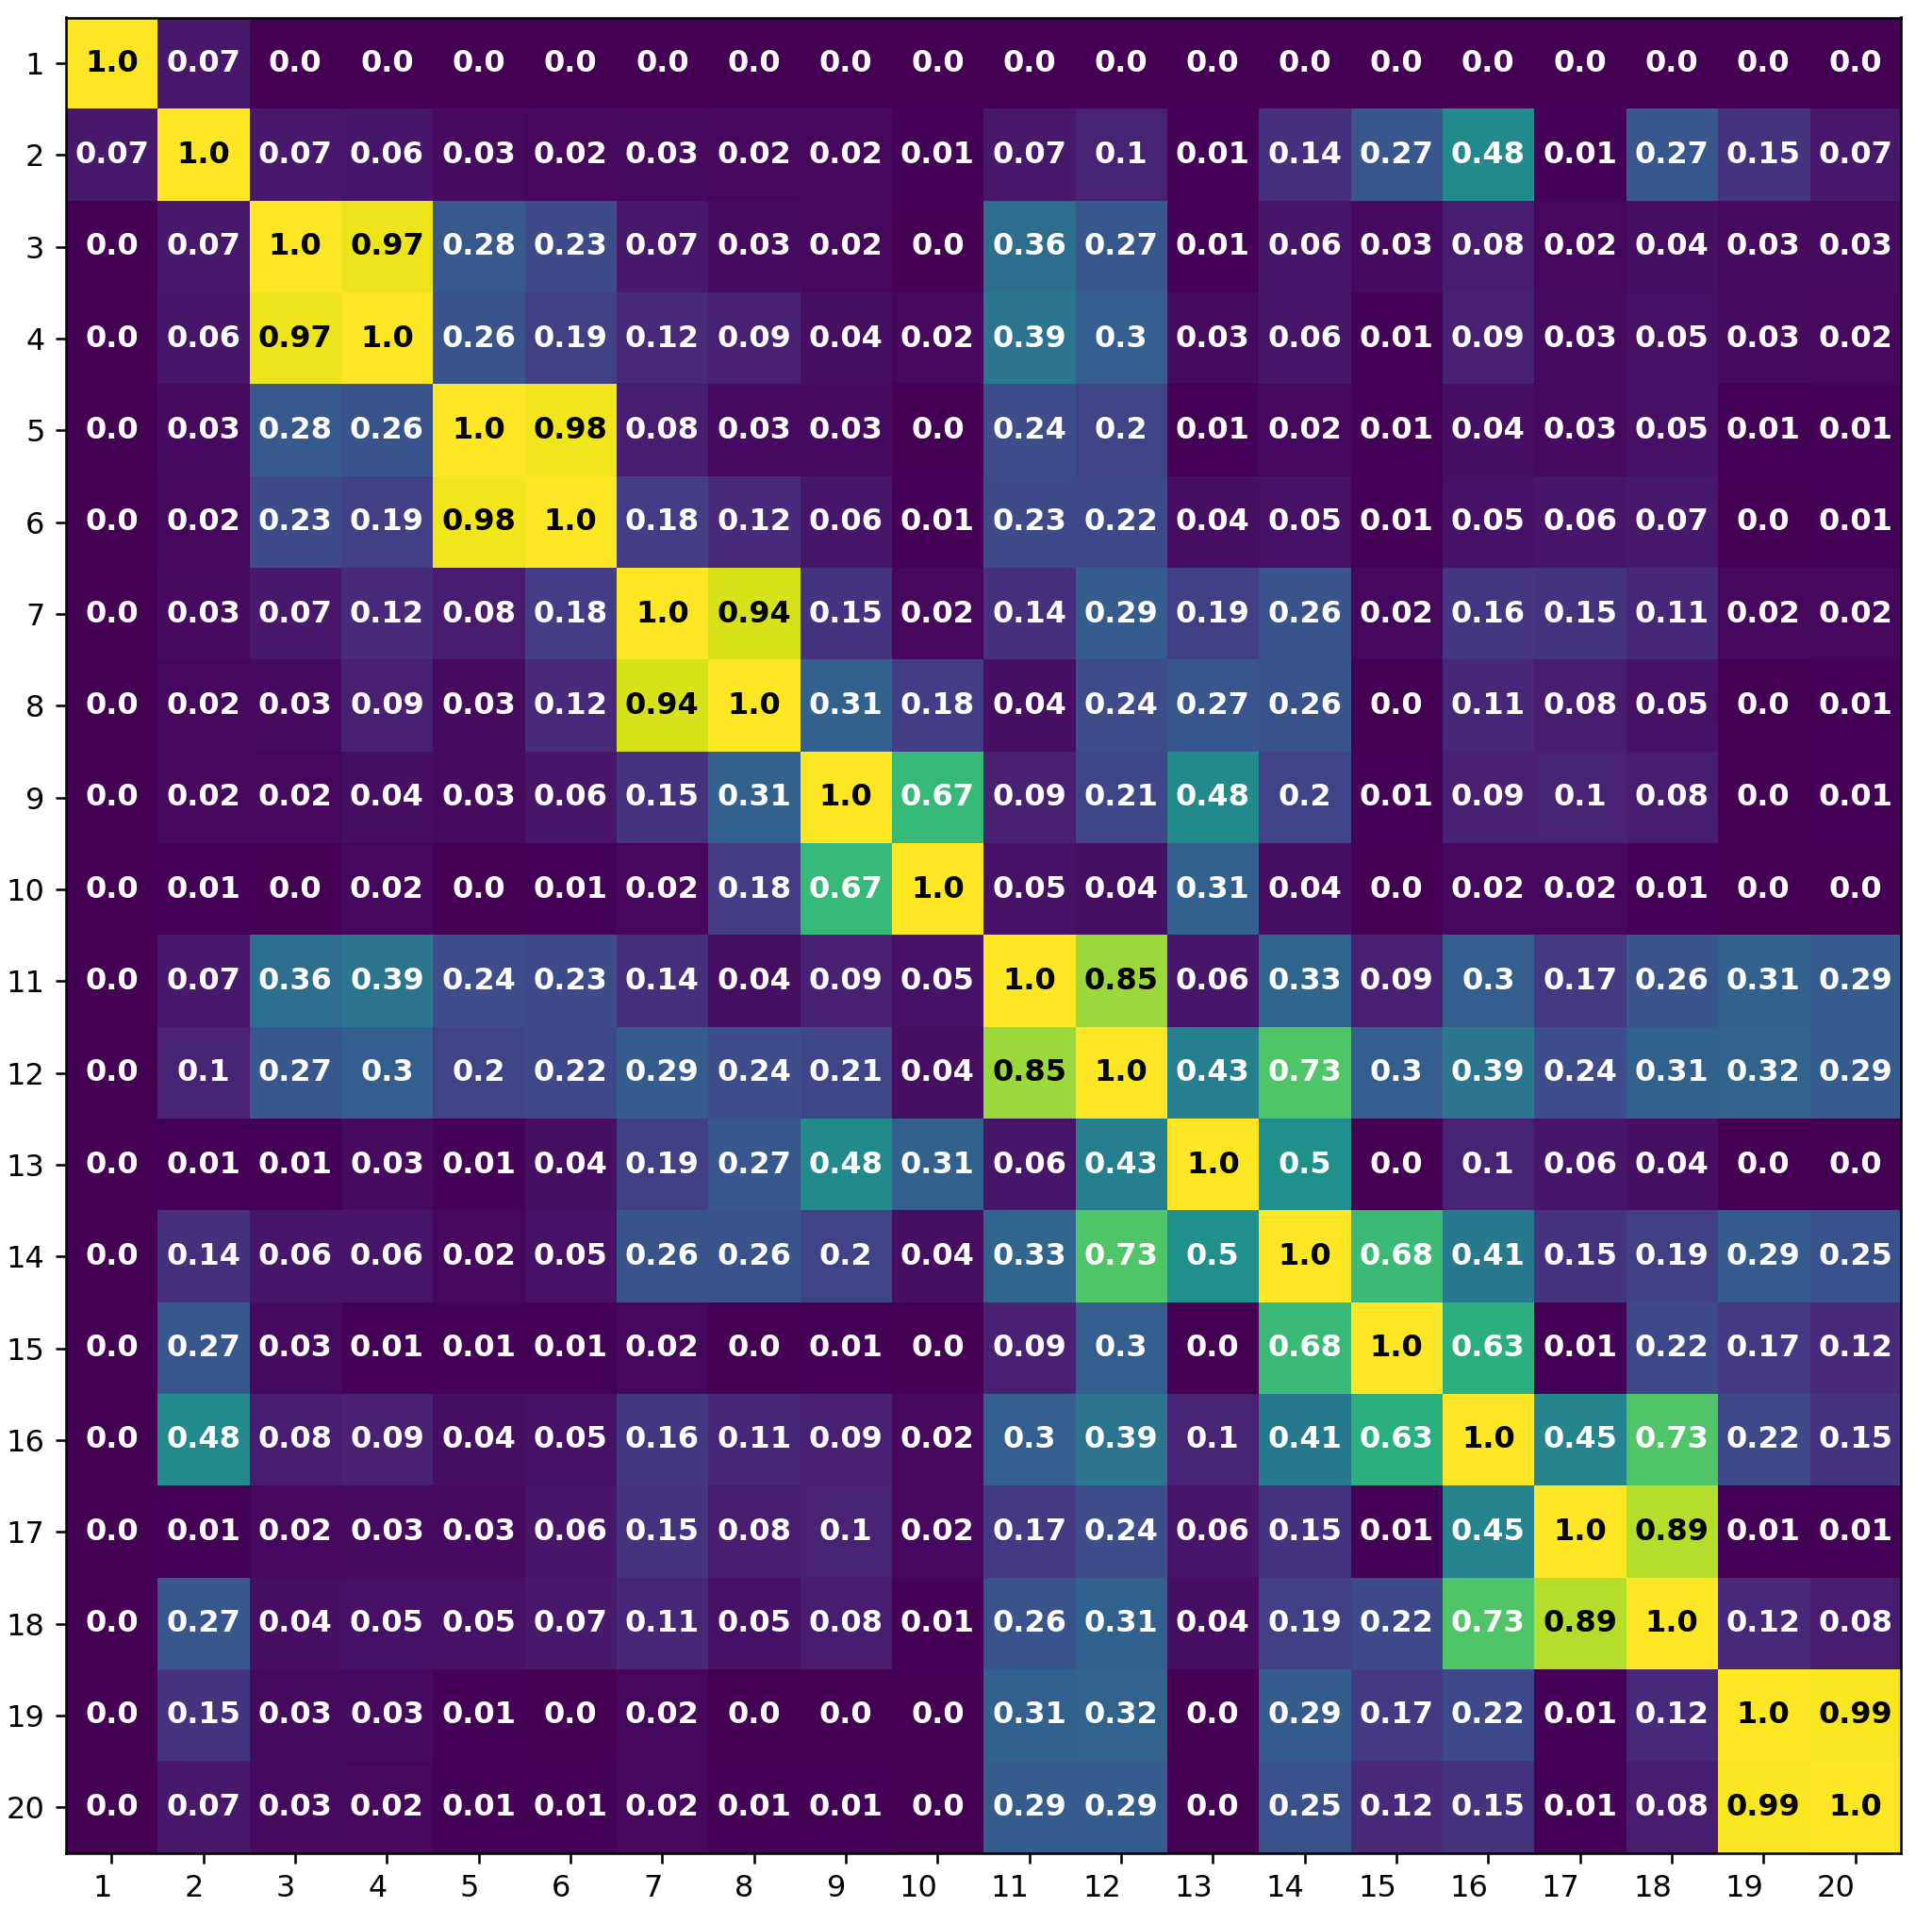
\includegraphics[width=16.5cm, height= 16.5cm]{ssa/W_corr.png}
	\caption{Корреляционная матрица компонент} \label{fig::W_corr_ssa}
\end{figure}

\noindent Финальным пунктом в примере классического SSA является демонстрация его предсказательных способностей.
\begin{figure}[H]
	\centering
	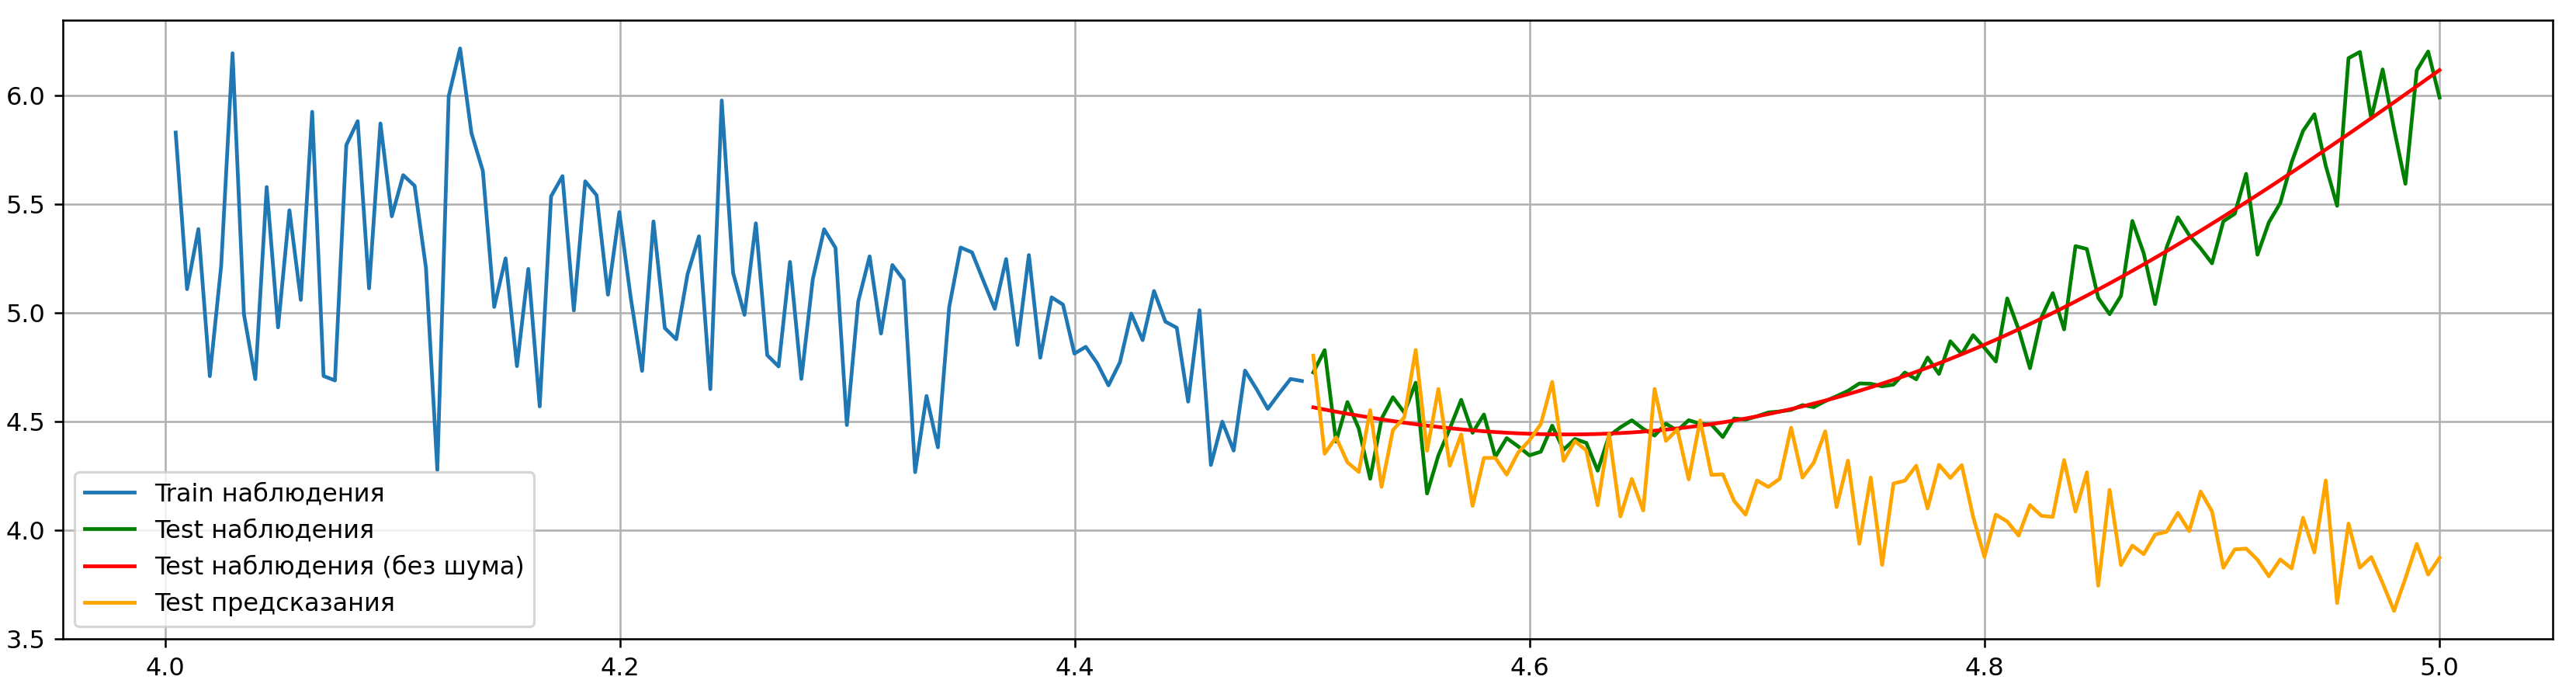
\includegraphics[width=16.5cm]{ssa/forecast_100.png}
	\caption{Прогнозирование значений $f(x)$ на ближайшие $100$ шагов}
\end{figure}
\noindent Анализируя полученные прогнозы, видим, что на начальных этапах они не очень плохи, однако дальше происходит расхождение самого тренда, что в случае с финансовыми рядами, влечет за собой большие риски (под риском понимается потеря денежного эквивалента из-за плохого расчета). Подобная ситуация случилась по 3-м причинам: 1) Малое количество компонент для деления 2) Отсутствие точного алгоритма группировки компонент 3) SSA не использует информацию о самом ряде, что анализирует, а опирается только на техническую составляющую. Однако 1) не говорит, что необходимо дробить ряд на как можно больше компонент, так как данный метод как и любой алгоритм требует как вычислительных мощностей, так и объемов оперативной памяти со стороны персонального компьютера. 2) не утверждает вообще ничего, а 3) упирается к гипотезу о рыночной эффективности и факт, что только техническим анализом невозможно точно предсказать поведение как цены, так и доходности актива соответственно \cite{fama_market_efficiency}. Конечно, 1-3 не утверждают, что SSA не применим вообще, иначе в чем смысл был смысл его создания. Решение - применять SSA конкретно для того, для чего он создавался: для анализа временных рядов - их декомпозиции и аппроксимации. то есть комбинировать его с другими алгоритмами, например, с NN или ARFIMA и так далее везде, где предсказывающая модель чувствительна к шуму в исходных данных. 

\subsubsubsection{Пример: Multistage SSA}
\\\\
Основываясь на алгоритме, предложенном в \cite{kuang2020efficient}, и используя данные, полученные посредством функции (\ref{link::illustr_func}), получаем эффект:
\begin{figure}[H]
	\centering
	\begin{tikzpicture}
		\begin{axis}[
			grid = both,
			legend pos = north west,
			minor tick num = 1,
			major grid style = {lightgray},
			minor grid style = {lightgray!25},
			%title= {},
			width = \textwidth,
			height = 0.45 \textwidth,
			xmin=-5, xmax=5,
			ymin=-4, ymax=7.5,
			line width=0.3mm
			]
			
			\addplot[color = orange, line width = 0.035cm] table [
			x=x, 
			y=denoised, 
			col sep=comma,
			mark={},
			] {./source/source_csv/Illustration data/ssa/denoised.csv};
			
			\addplot[opacity = 0.25, color = blue] table [
			x=x, 
			y=y, 
			col sep=comma,
			mark={},
			] {./source/source_csv/Illustration data/ssa/denoised.csv};
			
			\addplot[domain = -5:5,
			samples = 300,
			color = teal,
			smooth,
			line width = 0.025cm,] {sin(deg(5 * x)) + 1 / 4 * (x^2)};
			
			\legend{$\hat{f}(x)$ - оценка $f(x)$, $f(x)$ c шумом, $f(x)$ без шума};
		\end{axis}
	\end{tikzpicture}
	\caption{Очистка ряда от шума посредством MSSA}
\end{figure}
\noindent Да, очистка от шума не идеальная и существенные отличия от исходного (чистого) ряда, конечно, есть, однако, сравнивая с исходными данными, видим весьма ощутимое различие. Основываясь на этом, делаем вывод, что использование алгоритма MSSA в качестве непараметризованного метода очистки ряда, позволяет назвать сам предложенный метод весьма универсальным. Под <<универсальностью>> понимается отсутствие необходимости вмешательства человека в работу программы. То есть алгоритм делает все сам без помощи из вне. 

Более того, так как одной из основных задач настоящего исследования является написание программы, принимающей на вход некоторый временной ряд, а на выход дающей значение выбранной далее метрики качества для каждой из рассматриваемых моделей, универсальность метода MSSA также как и квази-универсальность (почти универсальность, закрывая глаза на малое количество гиперпараметров) позволяет использовать его в комбинации с другими алгоритмами прогнозирования, в которых конечное значение (прогноз) чувствителен к случайным шокам. Иными словами: очистка от шума необходимо там, где без нее нельзя обойтись для корректного обучения модели на тренировочных данных или там, где от шума возникают серьезные ошибки при построении прогноза. При этом отмечаем, что MSSA применяется только для удаления шума, а не для формирования прогноза как такового.

Таким образом, получаем, что вышеупомянутые алгоритмы очень интересны, функциональны и важны, так как сами по себе не являются зависимыми от некоторой экзогенно заданной модели. Включаем их в финальную таблицу.
		\subsubsubsection{Анализ Фурье} \label{link::fourier_analysis}
\\\\
\indent По изначальному подходу, сигнал $f(t)$ - это некоторая функция, то есть ее можно пытаться чем-то приближать. Конечно, далеко не всякую функцию можно аппроксимировать, однако пока что оставляем математическую строгость за кадром и просто пробуем. Но в таком случае из чего-то сложного как исходный сигнал, получаем что-то более простое, но поддающееся анализу, значит, мы раскладываем имеющуюся $f(t)$ на простые составляющие. Замечаем, что в первом приближении для этого должны быть выбраны простые функции, которые легко поддаются анализу. В таком случае, задаемся вопросом~\textbf{Q}: Можно ли как-то представить функцию вида $f(t)$ (исследуемый непрерывный сигнал) в виде конечного или бесконечного наложения синусоид (под синусоидой понимается как косинус, так и синус). \textbf{A}:~1)~Замечаем, что существует неточность: почему именно синусоиды? \textbf{Q}:~Почему нельзя взять иной набор функций, на которые раскладывается сигнал? \textbf{A}: Любой набор взять нельзя, однако при определенных условиях подобный подход приводит к рассматриваемому далее Wavelet анализу (\myref{link::wavelet_analysis}). На данный момент останавливаем рассуждения на  упоминании синусоид. Изначально было отмечено \cite{mipt2021string}, что струна - это тонкая и гибкая нить, способная совершать колебания при условии фиксированных концов как раз на основе синусоидальных форм. Причем по всей длине струны всегда умещается конечное количество волн. Это обеспечивается условием закрепленности струны на обоих концах. 

Самая простая форма колебания струны называется "гармоникой". Отсюда и происходит второе название анализа Фурье - гармонический анализ. Таким образом, формализуя исходную задачу, получаем выражение (\ref{equation::fourier_approximation}). Отмечаем, что факт того, как данное выражение изначально получено находится за областью, исследуемой в настоящей работе. Следовательно, предполагаем, что подобная форма разложения в ряд Фурье была <<угадана>>. 
\begin{equation} \label{equation::fourier_approximation}
	f(t) = \frac{a_0}{2} + \sum_{k = 1}^{\infty} a_k\cos(k \omega t) + b_k\sin(k \omega t)
\end{equation}
\indent Однако, несмотря на вольность предположений, далее совершенно строго находим для данного разложения все необходимые коэффициенты. Более того, отмечаем, что пока не было введено никаких предпосылок относительно $f(t)$, но далее они потребуются.

Пусть исходный сигнал $f(t)$ является периодическим с периодом $T$, тогда, основываясь на знаниях из Линейной Алгебры об ортогональных векторах, по аналогии вводим операцию <<измеряющую степень>> ортогональности функций~\cite{penn2016orthogonal}. В итоге получаем:
\begin{equation}
	p = \int_0^T g(t) f(t) \; \text{d}t
\end{equation}
\indent Далее вычисляем данную меру для выбранных в качестве базисных функций $\cos(\cdot)$ и $\sin(\cdot)$. Если $p \ne 0$, то вся проводимая операция не может быть названа разложением по базисным функциям. В силу того, что под <<синусоидой>> подразумевается как $\sin(\cdot)$, так и $\cos(\cdot)$, вычисляем меру $p$ для каждого из четырех возможных вариантов их комбинаций.
\begin{enumerate}
	\item $\sin(k\omega t), \sin(l \omega t): k, l \in \N, \omega \in \R^+$.
	\begin{equation}
		p = \int_{0}^T \sin(k\omega t)\sin(l \omega t) \; dt =
		\left\{
		\begin{array}{rl}
			0 & \text{, } k \ne l\\
			T / 2 & \text{, } k = l
		\end{array}
		\right.
	\end{equation}
	
	\item $\cos(k\omega t), \cos(l \omega t): k, l \in \N, \omega \in \R^+$.
	\begin{equation}
		p = \int_{0}^T \cos(k\omega t)\cos(l \omega t) \; dt =
		\left\{
		\begin{array}{rl}
			0 & \text{, } k \ne l\\
			T / 2 & \text{, } k = l
		\end{array}
		\right.
	\end{equation}
	
	\item $\cos(k\omega t), \sin(l \omega t): k, l \in \N, \omega \in \R^+$.
	\begin{equation}
		p = \int_{0}^T \cos(k\omega t)\sin(l \omega t) \; dt = 0
	\end{equation}
\end{enumerate}
Тогда, опираясь на  выражение (\ref{equation::fourier_approximation}) и умножение его обеих частей на $\sin(k\omega t)$ и $\cos(l \omega t)$, получаем формулы для коэффициентов. Рассматриваем только для $\sin(\cdot)$, так как аналогичным образом получается для $\cos(\cdot)$.
\begin{equation}
	\int_{0}^T f(t) \sin(p \omega t) dt = \int_0^T \sin(p \omega t) \left(\sum_{k = 1}^{\infty} a_k\cos(k \omega t) + b_k\sin(k \omega t) \right) dt
\end{equation}
Однако изменять порядок интегрирования и суммирования, при условии бесконечной суммы, можно только в случае равномерной сходимости ряда. Для настоящего ряда проблем в сходимости не наблюдается \cite{teljacovski2001convergence}, \cite{mipt2004fourier}. Преобразуем выражение, приняв во внимание факт ортогональности функций, описанный выше:
\begin{equation}
	\begin{split}
		\int_{0}^T f(t) \sin(p \omega t) \; dt & = \sum_{k = 1}^{\infty} b_k \int_0^T \sin(k \omega t)\sin(p \omega t) \; dt = T / 2  \cdot b_p \\
		b_k & = \frac{2}{T}  \int_{0}^T f(t) \sin(k \omega t) \; dt 
	\end{split}
\end{equation}
Аналогичным образом получаем выражение для коэффициентов $a_k$:
\begin{equation}
	a_k = \frac{2}{T}  \int_{0}^T f(t) \cos(k \omega t) \; dt 
\end{equation}
В более удобной форме вся задача приближения выглядит:
\begin{equation} \label{eq::fourier_task}
	\begin{split}
		f(t) & = \frac{a_0}{2} + \sum_{k = 1}^{\infty} a_k\cos(k \omega t) + b_k\sin(k \omega t)\\
		& = \frac{a_0}{2} + \sum_{k = 1}^{\infty} A_k \cos(k \omega t - \phi_k)\\
		A_k & = \sqrt{a_k^2 + b_k^2}\\
		\phi_k & = \arctan(b_k / a_k)\\
	\end{split}
\end{equation}
Где $A_k$ - амплитуда сигнала, а набор амплитуд $\left\{A_k\right\}_{k = 1}^\infty$ - спектр сигнала, $\phi_k$ - фаза сигнала. Переход к подобной записи как после 2-ого знака равенства сделан для того, чтобы было интуитивно удобнее характеризовать величину посредством не синуса и косинуса, а амплитуды и фазы в конкретный момент времени. Однако (\ref{eq::fourier_task}) можно еще больше упростить, перейдя в комплексную плоскость и воспользовавшись тождеством Эйлера:
\begin{equation}
	\exp(i k \omega t) = \cos(k \omega t) + i \sin(k \omega t)
\end{equation}
Отсюда получаем выражения для $\cos(k \omega t)$ и $\sin(k \omega t)$, после чего переписываем не все приближение, а только конкретный коэффициент $k$ (это сделано для удобства восприятия):
\begin{equation}
	\begin{split}
		a_k \cdot \frac{\exp(i k \omega t) + \exp(-i k \omega t)}{2} & + b_k \cdot \frac{\exp(i k \omega t) - \exp(-i k \omega t)}{2i}\\
		\underbrace{\left( \frac{a_k}{2} - \frac{b_k}{2} i \right) \exp(i k \omega t)}_{\text{<<Положительная>> часть}} & + \underbrace{\left( \frac{a_k}{2} + \frac{b_k}{2} i \right) \exp(-i k \omega t)}_{\text{<<Отрицательная>> часть}}
	\end{split}
\end{equation}
Отсюда получаем:
\begin{equation}
	c_k = \left\{
	\begin{array}{rl}
		a_k / 2 - i \cdot b_k/ 2  & \text{ ; } k \ge 0\\ 
		a_k / 2 + i \cdot b_k/ 2  & \text{ ; } k < 0\\ 
	\end{array}
	\right.
\end{equation}
В конечно виде (\ref{eq::fourier_task}) записывается уже как:
\begin{equation}
	f(t) = \sum_{k = -\infty}^{\infty} c_k \exp(i k \omega t)
\end{equation}
Однако тут интерес представляют сами коэффициенты $c_k$, так как именно они и являются коэффициентами Фурье при проецировании на базисные функции. 
\begin{equation}
	\begin{split}
		c_k & = \frac{a_k - i b_k}{2} = \frac{1}{\cancel{2}} \frac{\cancel{2}}{T} \int_0^T f(t) \cos(k \omega t) - f(t) \sin(k \omega t) \; dt\\
		& = \frac{1}{2 T} \int_{-T}^T f(t) \exp(-i k \omega t) \; dt
	\end{split}
\end{equation}
Вспоминаем, что ранее вводилась предпосылка, относительно периодичности сигнала $f(t)$. \textbf{Q}: Как быть в противном случае? \textbf{A}: Необходимо сам период устремить к $\infty$. Но прежде подставляем вместо некоторой частоты $\omega$ конкретное значение: $\omega = k \Delta \omega$, где $\Delta \omega = \pi / T$. Следовательно, $c_k = \langle f, \psi_k\rangle / (2 \pi)$, где $\psi_k \equiv \exp(i k t)$. Значит:
\begin{equation}
	\begin{split}
		f(t) & = \lim_{\Delta \omega \to 0} \sum_{k = -\infty}^{\infty} \frac{\Delta \omega}{2 \pi} \left[\int_{-\pi / \Delta \omega}^{\pi / \Delta \omega} f(\xi) \exp(-i k \Delta \omega \xi) \; d \xi\right] \exp(i k \Delta \omega)\\
	\end{split}	
\end{equation}
Но подобное выражение, путем вычисления предела, превращается в:
\begin{equation}
	\begin{split}
		f(t) & = \int_{-\infty}^{\infty} \frac{1}{2\pi} \underbrace{\left\{\int_{-\infty}^{\infty} f(\xi) \exp(-i \omega \xi) \; d \xi \right\}}_{\hat{f}(\omega)} \exp(i \omega t) \; d \omega\\
		f(t) & = \frac{1}{2 \pi} \int_{-\infty}^{\infty} \hat{f}(\omega) \exp(i \omega t) \; d\omega
	\end{split}
\end{equation}
Вывод: получаются формулы для прямого и обратного преобразования Фурье.
\begin{equation}
	\begin{split}
		\hat{f}(\omega) & = \mathcal{F}(f(t)) = \int_{-\infty}^{\infty} f(t) \exp(-i \omega t) \; dt\\
		f(t) & = \mathcal{F}^{-1}(\hat{f}(\omega)) = \frac{1}{2 \pi} \int_{-\infty}^{\infty} \hat{f}(\omega) \exp(i \omega t) \; d\omega
	\end{split}
\end{equation}
Таким образом, получаем возможность анализа функции в частотном пространстве. Однако стоит упомянуть, что преобразование Фурье имеет смысл применять только в случае стационарного спектра сигнала. То есть, как говорится в (\myref{def::signal_stationarity}), набор частот не должен меняться во времени. 

\begin{theorem}[теорема Персеваля \cite{brunton2022data}] \label{thm::parceval}
	<<Энергия>> исходного сигнала $f(t)$ (если он не является периодическим) или его <<сила>> (в случае периодичности) в пространстве времени $(t)$ равна данной величине, но в пространстве частот~$(\omega)$. 
	\begin{equation}
		\int_{\R} \lvert f(t) \rvert ^2 \; dt = \int_{\R} \lvert \hat{f}(\omega) \rvert ^2 \; d \omega
	\end{equation}
	В случае ненормированности базисной функции:
	\begin{equation}
		\lVert \hat{f} \rVert^2 = 2 \pi \lVert f \rVert^2 \Rightarrow \lVert \hat{f} \rVert^2 \propto \lVert f \rVert^2
	\end{equation}
	Где $\lVert f \rVert^2 = \int_{-\infty}^{\infty} \lvert f(t) \rvert^2 \; dt$.
\end{theorem}
Иными словами, данная теорема утверждает: если есть коэффициенты Фурье, которые достаточно малы (то есть по модулю близки к $0$), то <<удалив>> их (приравняв к $0$) получаем сигнал близкий к исходному $f(t)$.
		\subsubsubsection{Анализ wavelet} \label{link::wavelet_analysis}
\\\\
		\subsubsection{Neural Networks} \label{link::neural_networks}
	\subsubsubsection{Multilayer Perceptron}
	\subsubsubsection{Recurrent Neural Network}
	\subsubsubsection{Wavelet Network}
	\subsubsubsection{Алгоритмы обучения: GD семейство}
		